\documentclass[reprint, english,notitlepage,nofootinbib]{revtex4-1}  % defines the basic parameters of the document
% if you want a single-column, remove reprint

% allows special characters (including æøå)
\usepackage[utf8]{inputenc}
%\usepackage [norsk]{babel} %if you write norwegian
\usepackage[english]{babel}  %if you write english


%% note that you may need to download some of these packages manually, it depends on your setup.
%% I recommend downloading TeXMaker, because it includes a large library of the most common packages.

\usepackage{physics,amssymb}  % mathematical symbols (physics imports amsmath)
\usepackage{graphicx}         % include graphics such as plots

\usepackage[table]{xcolor}           % set colors
\usepackage{hyperref}         % automagic cross-referencing (this is GODLIKE)
\usepackage{tikz}             % draw figures manually
\usepackage{tikz-3dplot}
\usetikzlibrary{shapes,calc,positioning,intersections}
\tdplotsetmaincoords{80}{120}
%\usepackage[landscape]{geometry}
%\usepackage{expl3}
%\usepackage{xparse}
%\usepackage{pst-node}

\usepackage{listings}         % display code
\usepackage{subfigure}        % imports a lot of cool and useful figure commands
\usepackage{verbatim}
\usepackage{adjustbox}
\usepackage{dsfont}
\usepackage{mathtools}

% defines the color of hyperref objects
% Blending two colors:  blue!80!black  =  80% blue and 20% black
\hypersetup{ % this is just my personal choice, feel free to change things
    colorlinks,
    linkcolor={red!50!black},
    citecolor={blue!50!black},
    urlcolor={blue!80!black}}

%% Defines the style of the programming listing
%% This is actually my personal template, go ahead and change stuff if you want
\lstset{ %
	inputpath=,
	backgroundcolor=\color{white!88!black},
	basicstyle={\ttfamily\scriptsize},
	commentstyle=\color{magenta},
	language=Python,
	morekeywords={True,False},
	tabsize=4,
	stringstyle=\color{green!55!black},
	frame=single,
	keywordstyle=\color{blue},
	showstringspaces=false,
	columns=fullflexible,
	keepspaces=true}

\newcommand\numberthis{\addtocounter{equation}{1}\tag{\theequation}}
\newcommand{\ihat}{\boldsymbol{\hat{\textbf{\i}}}}
\newcommand{\jhat}{\boldsymbol{\hat{\textbf{\j}}}}
\newcommand{\khat}{\boldsymbol{\hat{\textbf{k}}}}
\newcommand{\ddpart}[2]{\frac{\partial #1}{\partial #2}}
\newcommand{\ddpartsq}[2]{\frac{\partial^2 #1}{\partial #2^2}}
\newcommand{\ddtot}[2]{\frac{\mathrm d #1}{\mathrm d #2}}
\newcommand{\ddtotsq}[2]{\frac{\mathrm d^2 #1}{\mathrm d #2^2}}
\newcommand{\vc}[1]{\mathbf{#1}}

\graphicspath{{../output/plots/}} % search for figures in this dir

\begin{document}


\begin{titlepage}
	\begin{center}
	\textbf{Diffusion Equation}

	\vspace{0.2cm}
	Vegard Falmår and Sigurd Sørlie Rustad

	\vspace{0.5cm}
	
\includegraphics[scale=0.5]{../../pictures/UIO}
	\vspace{0.8cm}

	University of Oslo\\
	Norway\\
	\today	\\
	\end{center}
	\tableofcontents
	\clearpage
\end{titlepage}

\begin{abstract}
  note to self: kanskje ikke helt fornøyd med siste del av metode 1D og 2D? si noe om stability i 2D? Ellers burde alt være ganske nais. Unit testing mangler. diskutere at de første tidsstegene så er computed best? Derfor ser vi på midt i og stationary state.
\end{abstract}
\maketitle                              % creates the title


\section{Introduction}
The diffusion equation is used in many areas. Everything from how heat is transferred through a stick, to how an oil spill will spread. In this report we will try to solve the diffusion equation for one and two dimensions, and using different algorithms. We are going to study the diffusion equation with a constant collective diffusion coefficient, giving us a linear differential equation identical to the heat equation.

For our one dimensional problem, we use three different algorithms, explicit Forward Euler, implicit Backward Euler and implicit Crank-Nicolson.

For our studies we have used c++ for heavy computation, python for visualization and automation. All the code along with instructions on how to run it, can be cloned from our GitHub repository\footnote{github.com/sigurdru/FYS3150/tree/master/Project5}.

\section{Theory}

\subsection*{The diffusion equation}

The full diffusion equation reads
\begin{equation*}
	\frac{\partial u(\mathbf{r}, t)}{\partial t} = \nabla \cdot \left[D(u, \mathbf{r})\nabla u(\mathbf{r}, t)\right],
\end{equation*}
where $\mathbf{r}$ is a positional vector and $D(u,r)$ the collective diffusion coefficient. If $D(u,\mathbf{r}) = 1$ the equation simplifies to a linear differential equation
\begin{equation*}
	\frac{\partial u}{\partial t} = \nabla^2u(\mathbf{r}, t),
\end{equation*}
or
\begin{equation}
	\label{eq:diffusion_equation}
	\left(\frac{\partial^2}{\partial x^2} + \frac{\partial^2}{\partial y^2} + \frac{\partial^2}{\partial z^2}\right) u(x,y,z,t) = \frac{\partial u(x,y,z,t)}{\partial t}
\end{equation}
in cartesian coordinates. In this report we are mainly going to work with the diffusion equation in one and two dimensions, i.e.
\begin{align*}
	 \frac{\partial^2 u(x,t)}{\partial x^2} &= \frac{\partial u(x,t)}{\partial t} \\ &\wedge \\ \frac{\partial^2u(x, y,t)}{\partial x^2} + \frac{\partial^2u(x, y,t)}{\partial y^2} &= \frac{\partial u(x, y,t)}{\partial t}.
\end{align*}

\subsection*{Mean absolute percentage error}

The mean absolute percentage error (MAPE), is used to predict the accuracy of a prediction. We will use it to measure how good our numerical methods are, compared to theoretical values. Equation \eqref{eq:MAPE} shows how to calculate MAPE in percentage,
\begin{equation}
	\label{eq:MAPE}
	M = \left(\frac{1}{n}\sum_{n=1}^{n}\abs{\frac{A_\text{t} - A_\text{c}}{A_\text{t}}}\right)\cdot 100\%.
\end{equation}
Here $A_\text{t}$ and $A_\text{c}$ are the theoretical and computed values, $n$ number of data points and $M$ MAPE in percent.

\subsection*{Discretization}

Equation \eqref{eq:diffusion_equation} in one dimension reads
\begin{equation}
\label{eq:diffusion_equation_1D}
\frac{\partial^2u(x, t)}{\partial x^2} = \frac{\partial u(x,t)}{\partial t} \ \ \text{or} \ \ u_{xx} = u_t.
\end{equation}
With $x\in[0,L]$ and boundary conditions
\begin{equation*}
\label{eq:boundary_conditions}
u(0, t) = a(t), \ \ t\geq 0 \ \ \wedge \ \ u(L,t) = b(t), \ \ t\geq 0,
\end{equation*}
we can approximate the solution by discretization. First introducing $\Delta x = L/(n+1)$ and $\Delta t$ as small steps in $x$-direction and time. Then we can define the value domain of $t$ and $x$,
\begin{equation*}
t_j = j\Delta t, \ \ j\in \mathbb{N}_0 \ \ \wedge \ \ x_i = i\Delta x, \ \ \{i \in \mathbb{N}_0 | i \leq n + 1\}.
\end{equation*}

\subsection*{Explicit and implicit schemes}

It is common to divide numerical algorithms into explicit and implicit schemes. When performing numerical integration, we iterate over a discrete set of grid points at which we evaluate the function in question. In explicit schemes, the value at the next grid point is determined entirely by known or previously calculated values. In implicit schemes, the value is determined by solving a coupled set of equations, often involving matrix or iterative techniques.

Using an implicit method instead of an explicit method usually requires more computation in every step, and they are often harder to implement. It can, in turn, save computation by allowing larger step sizes. Explicit methods are always conditionally stable, however the implicit methods we will use in this report are unconditionally stable. Of course, in order to achieve a desired \textit{accuracy}, the step sizes can not be arbitrarily large for either the explicit or implicit schemes. It is generally the case, though, that implicit schemes allow for larger step sizes than explicit schemes.

\subsection*{Explicit Forward Euler}

The algorithm for explicit forward Euler in one dimension (from \cite{lectures2015} chapter 10.2.1) reads
\begin{equation}
  \label{eq:forward_euler}
	u_{i, j+1} = \alpha u_{i-1, j} + (1 - 2\alpha) u_{i,j} + \alpha u_{i+1, j}
\end{equation}
where
\begin{equation*}
	\alpha = \frac{\Delta t}{\Delta x^2},
\end{equation*}
and a local approximate error of $O(\Delta t)$ and $O(\Delta x ^2)$. The discretization is explained in the appropriate section. Note that the expression on the right hand side, used to calculate the value at a time $t_j + \Delta t$, only contains the state of the system at time $t_j$. This can be written as a matrix equation (see \cite{lectures2015} chapter 10.2.1)
\begin{equation*}
	\mathbf{u}_{j+1} = (\mathds{1} - \alpha \mathbf{B})\mathbf{u}_j
\end{equation*}
where $\mathds{1}$ is the identity matrix and
\begin{equation*}
	\begin{bmatrix}
	2 & -1 & 0 & 0\dots \\
	-1 & 2 & -1 & 0\dots\\
	\dots & \dots & \dots &\dots \\
	0 & \dots & -1 & 2
	\end{bmatrix}	 \ \ \wedge \ \
	\mathbf{u}_{j} = \begin{bmatrix}
	u_{1,j} \\
	u_{2,j} \\
	\ldots \\
	u_{n,j}
	\end{bmatrix}
\end{equation*}
The stability requirement for this algorithm (also from \cite{lectures2015} chapter 10.2.1) is
\begin{equation}
	\label{eq:von_neumann_stability}
	\rho(\mathbf{B}) \le 1 \implies \frac{\Delta t}{(\Delta x)^2} \le 1/2
\end{equation}
Where $\rho(\mathbf{B})$ is the spectral radius of $\mathbf{B}$:
\begin{equation*}
	\rho(\mathbf{B}) = \text{max}\{|\lambda|:\text{det}(\mathbf{B}- \lambda \mathds{1}) = 0\}.
\end{equation*}

In two dimensions ($u(x,y)$) the method for solving is similar. Assuming the same number of integration points in x- and y-direction ($\Delta x = \Delta y = \Delta l$), the algorithm (from \cite{lectures2015} chapter 10.2.5) reads
\begin{equation}
	\label{eq:3dEuler}
	u_{i,j}^{l+1} = u_{i,j}^{l} + \alpha \left[u_{i+1,j}^{l} + u_{i-1,j}^{l} + u_{i,j+1}^{l} + u_{i,j-1}^{l} - 4u_{i,j}^{l}\right]
\end{equation}
where $u_{i,j}^l = u(i\Delta l, j \Delta l, l\Delta t)$ and $\alpha = \Delta t/\Delta l^2$. With this algorithm we will get slightly different stability conditions. The Von Neumann stability analysis gives
\begin{equation}
	\label{eq:2D_von_neumann_stability}
	\frac{\Delta t}{\Delta l^2} \leq \frac{1}{4}
\end{equation}
see \cite{MiT} for derivation.


\subsection*{Implicit Backward Euler}

The Backward Euler algorithm uses the same centered difference in space as Forward Euler to approximate the second derivative
\begin{equation}
  \label{eq:centered_2nd_deriv_space}
	u_{xx} \approx \frac{u(x_i + \Delta x, t_j) - 2u(x_i,t_j) + u(x_i-\Delta x, t_j))}{\Delta x^2},
\end{equation}
but a backward formula for the time derivative:
\begin{equation}
  \label{eq:backward_deriv_time}
  u_t \approx \frac{u(x_i, t_j) - u(x_i, t_j - \Delta t)}{\Delta t},
\end{equation}
which also has a local truncation error of $O(\Delta t)$ and $O(\Delta x ^2)$.
Again, defining
\begin{equation*}
  \alpha = \frac{\Delta t}{(\Delta x)^2}
\end{equation*}
we obtain by inserting \eqref{eq:centered_2nd_deriv_space} and \eqref{eq:backward_deriv_time} into our differential equation the equation describing Backward Euler:
\begin{equation}
  \label{eq:backward_euler}
  u_{i, j-1} = -\alpha u_{i-1, j} + (1 + 2 \alpha) u_{i, j} - \alpha u_{i+1, j}
\end{equation}

Written out for all $i$, equation \ref{eq:backward_euler} becomes
\begin{align*}
  - \alpha u_{0, j} + (1 + 2 \alpha) u_{1, j} - \alpha u_{2, j} &= u_{1, j-1} \\
  - \alpha u_{1, j} + (1 + 2 \alpha) u_{2, j} - \alpha u_{3, j} &= u_{2, j-1} \\
  ... \\
  - \alpha u_{n-3, j} + (1 + 2 \alpha) u_{n-2, j} - \alpha u_{n-1, j} &= u_{n-2, j-1} \\
  - \alpha u_{n-2, j} + (1 + 2 \alpha) u_{n-1, j} - \alpha u_{n, j} &= u_{n-1, j-1} \\
\end{align*}
In general, this can be rearranged slightly so that
\begin{align*}
  (1 + 2 \alpha) u_{1, j} -\alpha  u_{2, j} &= u_{1, j-1} + \alpha u_{0, j} \\
  - \alpha u_{1, j} + (1 + 2 \alpha) u_{2, j} - \alpha u_{3, j} &= u_{2, j-1} \\
  ... \\
  - \alpha u_{n-3, j} + (1 + 2 \alpha) u_{n-2, j} - \alpha u_{n-1, j} &= u_{n-2, j-1} \\
  - \alpha u_{n-2, j} + (1 + 2 \alpha) u_{n-1, j} &= u_{n-1, j-1} + \alpha u_{n, j} \\
\end{align*}
Let $\vc v_j$ be a vector containing the values of $u$ at $n - 1$ points in space at a time $t_j$
\begin{equation}
  \label{def:vector_v}
  \vc v_j =
  \begin{bmatrix}
    u_{1, j} \\
    u_{2, j} \\
    \vdots \\
    u_{n-2, j} \\
    u_{n-1, j} \\
  \end{bmatrix}
\end{equation}
and the vector $\vc b_j$ be defined as follows:
\begin{equation}
  \label{def:vector_b_BackwardEuler}
  \vc b_j =
  \begin{bmatrix}
    u_{1, j-1} + \alpha u_{0, j} \\
    u_{2, j-1} \\
    \vdots \\
    u_{n-2, j-1} \\
    u_{n-1, j-1} + \alpha u_{n, j} \\
  \end{bmatrix}
\end{equation}
As the boundary conditions $u_{0, j}$ and $u_{n, j}$ are specified, we already know every component of $\vc b_j$. We can then rewrite equation \eqref{eq:backward_euler} as the matrix equation
\begin{equation}
  \label{eq:backward_euler_matrix}
  \vc A \vc v_j = \vc b_j
\end{equation}
where $\vc A$ is defined as
\begin{equation}
  \label{def:matrix_A}
  A =
  \begin{bmatrix}
    (1 + 2 \alpha) & -\alpha         & 0       & 0      & \ldots         & 0 \\
    -\alpha        & (1 + 2 \alpha)  & -\alpha & 0      & \ldots         & 0 \\
    \vdots         &                 & \ddots  &        &                & \vdots \\
    0              & \ldots          & 0       &-\alpha & (1 + 2 \alpha) & -\alpha  \\
    0              & \ldots          & 0       & 0      &-\alpha         & (1 + 2 \alpha)  \\
  \end{bmatrix}
\end{equation}
This is a tridiagonal matrix with $(1 + 2 \alpha)$ on the diagonal and $-\alpha$ directly above and below the diagonal.


\subsection*{Implicit Crank-Nicolson}

The Crank-Nicolson algorithm uses a time-centered scheme centered around $t + \Delta t/2$, with a truncation error of $O(\Delta t^2)$ and $O(\Delta x^2)$. The time derivative is given by
\begin{equation}
  \label{eq:forward_deriv_time}
  u_t \approx \frac{u(x_i, t_j + \Delta t) - u(x_i, t_j)}{\Delta t}
\end{equation}
\begin{align*}
	u_{xx} &\approx \frac{1}{2 \Delta x^2} \bigg(u(x_i+\Delta x, t_j) - 2u(x_i,t_j) + u(x_i-\Delta x, t_j) \\
  	&\quad + u(x_i+\Delta x, t_j + \Delta t) - 2u(x_i, t_j + \Delta t) \\
  	&\quad + u(x_i - \Delta x, t_j + \Delta t) \bigg)
\end{align*}

Inserting these two equations into our differential equation, we obtain (see Appendix, section \ref{sect:Crank-Nicolson_derivation} for derivation) that the equation describing the Crank-Nicolson algorithm can be written as a matrix equation
\begin{equation}
  \label{eq:Crank-Nicolson_matrix}
  \vc A \vc v_j = \vc b_j
\end{equation}
The vector $\vc v_j$ is the same as in the case of Backward Euler, defined in \eqref{def:vector_v}. The matrix $\vc A$ is a tridiagonal matrix with $2 (1 + \alpha)$ on the diagonal and $-\alpha$ directly above and below the diagonal. The vector $\vc b_j$ is
\begin{equation}
  \label{def:vector_b_CrankNicolson}
  \vc b_j =
  \begin{bmatrix}
    \alpha u_{0, j-1}  + 2 (1 - \alpha) u_{1,j-1} + \alpha u_{2, j-1} + \alpha u_{0, j} \\
    \alpha u_{1, j-1}  + 2 (1 - \alpha) u_{2,j-1} + \alpha u_{3, j-1} \\
      \vdots \\
    \alpha u_{n-3, j-1}  + 2 (1 - \alpha) u_{n-2,j-1} + \alpha u_{n-1, j-1} \\
    \alpha u_{n-2, j-1}  + 2 (1 - \alpha) u_{n-1,j-1} + \alpha u_{n, j-1} + \alpha u_{n, j}
  \end{bmatrix}
\end{equation}



\section{Methods}

\subsection{One dimension}
We will start by solving the one dimensional diffusion equation
\begin{equation*}
  \frac{\partial^2 u(x,t)}{\partial x^2} = \frac{\partial u(x,t)}{\partial t}, \quad x \in [0, 1]
\end{equation*}
with initial conditions
\begin{equation}
	\label{eq:1D_init}
  u(x, 0) = 0, \quad 0<x<1\\
\end{equation}
and boundary conditions
\begin{align}
	\label{eq:1D_bound}
	\begin{split}
  u(0, t) &= 0, \quad t \ge 0 \quad \text{and} \\
  u(L, t) &= 1, \quad t \ge 0.
  \end{split}
\end{align}
As mentioned we use three methods, explicit forward Euler, implicit backward Euler and Crank-Nicolson. When using Explicit forward Euler, we only need to solve the difference-equation described by equation \eqref{eq:forward_euler}. When using Implicit backward Euler er Crank-Nicolson we need to solve the matrix-equations \eqref{eq:backward_euler_matrix} and \eqref{eq:Crank-Nicolson_matrix}. There are several methods for solving such tridiagonal matrix equations, however we will use the method covered in a previous project. see project\footnote{https://github.com/sigurdru/FYS3150/tree/master/Project1} page 2 (section A. Solve tridiagonal matrix equation). We will use $\Delta x = 1/10$, $\Delta x = 1/100$ and $\Delta t$ decided by equation \eqref{eq:von_neumann_stability}. We then study compare our results with analytical ones (analytical results are derived below), at two points in time. First $t_1$ where our solution is smooth but curved, then $t_2$ where we have a linear (stable) solution. Hopefully we will be able to decide on what method is best. We also check what happens when the difference in equation \eqref{eq:von_neumann_stability} is not satisfied. For all our results we also plot the difference between the results, as well as calculate the MAPE in percent (see equation \eqref{eq:MAPE}).

\subsection*{Analytic solution to the 1D diffusion equation}

With the initial and boundary conditions described by equations \eqref{eq:1D_init} and \eqref{eq:1D_bound} we can find an analytical solution. We expect the heat distribution to converge to a stable state $u_E$ as $t \to \infty$:
\begin{equation*}
\lim_{t \to \infty} u(x, t) = u_E(x)
\end{equation*}
This final state should still satisfy our differential equation such that
\begin{equation*}
\frac{\partial^2 u_E(x)}{\partial x^2} = \ddpart{u_E(x)}{t} = 0
\end{equation*}
The solution to this equation is
\begin{equation*}
u_E(x) = A x + B,
\end{equation*}
and the boundary conditions give
\begin{align*}
u_E(0) &= B = 0 \\
u_E(L) &= A L = 1 \quad \Rightarrow \quad u_E(x) = \frac{x}{L}
\end{align*}

Let us now define the function
\begin{align*}
v(x, t) &= u(x, t) - u_E(x) \quad \text{which gives} \\
u(x, t) &= v(x, t) + u_E(x)
\end{align*}
We then have
\begin{align*}
\ddpart{u}{t} &= \ddpart{v}{t} + \ddpart{u_E}{t} = \ddpart{v}{t} \\
\ddpartsq{u}{x} &= \ddpartsq{v}{x} + \ddpartsq{u_E}{x} = \ddpartsq{v}{x}
\end{align*}
Thus, $u(x, t)$ and $v(x, t)$ should both satisfy the same differential equation \eqref{eq:diffusion_equation_1D}. The intial and boundary conditions for $v(x, t)$ are
\begin{align*}
v(x, 0) &= u(x, 0) - u_E(x) = - u_E(x) \\
v(0, t) &= u(0, t) - u_E(0) = 0 \\
v(0, t) &= u(L, t) - u_E(L) = 0
\end{align*}
In other words, $v$ obeys the same equation as $u$, but with boundary conditions 0.

It is rather straightforward to see that (however see \cite{PDE_book} chapter 3 for a more thorough derivation)
\begin{equation}
\label{eq:analytic_part_sol_1D_diffusion_general}
f_n(x, t) = e^{- C_n^2 t} \left( A \sin(C_n x) + B \cos(C_n x) \right)
\end{equation}
is a particular solution to the one dimensional diffusion equation:
\begin{equation*}
\frac{\partial f_n(x, t)}{\partial t} = \frac{\partial^2 f_n(x, t)}{\partial x^2} = -C_n^2 f_n(x, t)
\end{equation*}
The equation is linear and from the prinsiple of superposition we have that any sum of functions $f_n(x, t)$ with different values of $C_n$ is also a solution. The boundary conditions $v(0, t) = 0$ and $v(L, t) = 0$ give
\begin{align*}
f_n(0, t) &= B_n e^{- C_n^2 t} = 0 \quad \Rightarrow \quad B_n = 0 \\
f_n(L, t) &= A_n e^{- C_n^2 t} \sin(C_n L) = 0 \quad \Rightarrow \quad C_n = \frac{n \pi}{L}, n \in \mathbb{Z}
\end{align*}
The solution $v(x, t)$ can then be written as sum
\begin{equation*}
v(x, t) = \sum_n A_n e^{- \left( \frac{n \pi}{L} \right)^2 t} \sin( \frac{n \pi}{L} x)
\end{equation*}
The coefficients $A_n$ are given by the initial condition $v(x, 0) = - u_E(x)$ and can be determined from (see \cite{lectures2015} chapter 10.2.4)
\begin{align*}
A_n &= \frac{2}{L} \int_0^L - u_E(x) \; \sin( \frac{n \pi}{L} x) \; \mathrm dx \\
&= - \frac{2}{L^2} \int_0^L x \; \sin( \frac{n \pi}{L} x) \; \mathrm dx
\end{align*}
The solution to this is
\begin{equation}
\label{eq:fourier_coeffs}
A_n = \dfrac{2 \left( \pi n \cos(\pi n) - \sin(\pi n) \right)}{\pi^2 n^2}
\end{equation}

The complete solution to our differential equation is thus
\begin{equation}
\label{eq:exact_solution_1D}
u(x, t) = \frac{x}{L} + \sum_{n=1}^\infty A_n e^{- \left( \frac{n \pi}{L} \right)^2 t} \sin( \frac{n \pi}{L} x),
\end{equation}
where the coefficients $A_n$ are given by equation \eqref{eq:fourier_coeffs}.

\subsection{Two dimensions}
Moving on to two dimensions we use explicit forward Euler. This means we need to solve the difference equation \eqref{eq:3dEuler}, for $x, y \in [0,1]$. We will use homogeneous Dirichlet boundary conditions
\begin{align}
	\label{eq:2D_bound}
	\begin{split}
	u(0, y, t) &= u(1, y, t) = 0, \quad 0\leq y \leq 1, \ \ t\geq 0 \text{ and}\\
	u(x, 0, t) &= u(x, 1, t) = 0, \quad 0\leq x \leq 1, \ \ t\geq.
	\end{split}
\end{align}
and initial conditions given by
\begin{equation}
\label{eq:2D_init}
	u(x,y,0) =
	\begin{cases}
	1\quad \text{if }0<y\leq \frac{1}{2}\text{ and } 0<x<1 \\
	0\quad \text{if }\frac{1}{2}<y<1\text{ and } 0<x<1
	\end{cases}
\end{equation}
As for the one we will test for different $\Delta t$'s, and compare it to the closed form solution covered bellow. We do one case where the difference in equation \eqref{eq:2D_von_neumann_stability} is satisfied and one where it's not. We then plot the result and difference between them, also calculating MAPE in percent (equation \eqref{eq:MAPE}). For all cases we used $\Delta x= \Delta y = 1/50$.

\subsection*{Parallelization}
When solving the difference equation \eqref{eq:3dEuler} we parallelize the program using OpenMp. While calculating $u_{i,j}^l$ we only need to worry about the surrounding points for the previous step, namely $u_{i,j}^{l-1}$ and $u_{i\pm 1,j\pm 1}^{l-1}$. In a grid pattern this would look something like:
\begin{equation*}
\scalebox{1.5}{
	$\begin{matrix}
	& u_{i,j+1}^{l-1} & \\
	\\
	u_{i-1,j}^{l-1} & u_{i,j}^{l-1} & u_{i+1,j}^{l-1} \\
	\\
	& u_{i,j-1}^{l-1} &
	\end{matrix}$}
\end{equation*}
This means that whenever we are done calculating $u_{i,j}^{l}$ and $u_{i\pm 1,j\pm 1}^{l}$ we can start calculating the next time step $u_{i,j}^{l+1}$. We found that if we run through $u_{i,j}^{l}$ diagonally, we can start calculating the next time step ($u_{i,j}^{l+1}$) one diagonal behind. A visual representation of this can be seen in figure \ref{fig:parallelization}. The red and black dots represent values of $u_{i,j}^l$ we have and haven't calculated respectively. We can then make sure one thread is calculating $u_{i,j}^l$ for one value of $l$ diagonally, another core the next time step one diagonal behind, and so forth.
We will be timing our code for a selected few runs to determine the effect of parallelization.

\begin{figure}[!h]
	\textbf{\scalebox{1.2}{Representation of $\mathbf{u}_{i,j}^l$}}\par\medskip
\begin{tikzpicture}[scale=2.5, tdplot_main_coords,axis/.style={->},thick]

\foreach \x in {0,1,2}
\foreach \y in {0,1,2}
\foreach \z in {0,1,2}
{
	\draw[thick,opacity=1] (\x,0,\z) -- (\x,2,\z);
	\draw[thick,opacity=1] (0,\y,\z) -- (2,\y,\z);
	\draw[thick,opacity=1] (\x,\y,0) -- (\x,\y,2);
}

\draw (2.5,0,1) node[below] {\Large $l \rotatebox{90}{$\xrightarrow{\makebox[2cm]{}}$}$};
\draw (1,0,0.45) node[below] {\Large $j
\rotatebox{18}{$\xrightarrow{\makebox[1.5cm]{}}$}$};
\draw (1.5,0.4,-0.1) node[below] {\Large $i
\rotatebox{-8}{$\xrightarrow{\makebox[1.5cm]{}}$}$};

% --- labels for vertices
\foreach \x in {0,1,2}
\foreach \y in {0,1,2}
\foreach \z in {0,1,2}
{\draw[fill=red] (\x,\y,\z) circle (0.3em);}
%top level
\foreach \x in {0,1}
\foreach \y in {0,1,2}
\foreach \z in {2}
{\draw[fill=black] (\x,\y,\z) circle (0.3em);}

\foreach \x in {2}
\foreach \y in {1,2}
\foreach \z in {2}
{\draw[fill=black] (\x,\y,\z) circle (0.3em);}
%middle level
\foreach \x in {0,1,2}
\foreach \y in {2}
\foreach \z in {1}
{\draw[fill=black] (\x,\y,\z) circle (0.3em);}

\foreach \x in {0,1}
\foreach \y in {1}
\foreach \z in {1}
{\draw[fill=black] (\x,\y,\z) circle (0.3em);}

\foreach \x in {0}
\foreach \y in {0}
\foreach \z in {1}
{\draw[fill=black] (\x,\y,\z) circle (0.3em);}

%bottom level
\foreach \x in {0,1}
\foreach \y in {2}
\foreach \z in {0}
{\draw[fill=black] (\x,\y,\z) circle (0.3em);}

\foreach \x in {0}
\foreach \y in {1}
\foreach \z in {0}
{\draw[fill=black] (\x,\y,\z) circle (0.3em);}

\end{tikzpicture}
\caption{Visualization of how the parallelization works. $i$, $j$ and $l$ represent the indexes of $u_{i,j}^{l}$ and the red and black dots represent the values of $u_{i,j}^{l}$ we have and haven't calculated.
\label{fig:parallelization}}
\end{figure}

\subsection*{Analytical solution to the 2D diffusion equation}
with boundary and initial conditions described by equations \eqref{eq:2D_bound} and \eqref{eq:2D_init} we can find analytical solutions to the diffusion equation. Lets say $x\in[0,a]$ and $y\in[0,b]$, with homogeneous Dirichlet boundary and initial conditions defined by some function $f(x,y)$. Then, from \cite{2D_diffusion}, the general solution is given by equation \eqref{eq:2D_gen_sol}.
\begin{equation}
	\label{eq:2D_gen_sol}
	u(x,y,t) = \sum_{m=1}^{\infty}\sum_{n=1}^{\infty}A_{mn}\sin(\mu_m x)\sin(\nu_n y)e^{-\lambda^2_{mn}t},
\end{equation}
where
\begin{equation*}
	\mu_m = \frac{m\pi}{a} \ \ \wedge \ \ \nu_n=\frac{n\pi}{b} \ \ \wedge \ \ \lambda_{mn} = \sqrt{\mu_m^2 + \nu_n^2},
\end{equation*}
for $m,n,\in\mathbb{N}$ and
\begin{equation*}
	A_{mn} = \frac{4}{ab}\int_{0}^{a}\int_{0}^{b}dydxf(x,y)\sin(\frac{m\pi}{a}x)\sin(\frac{n\pi}{b}).
\end{equation*}
Inserting our initial conditions \eqref{eq:2D_init} and $a=b=1$ into the equation above, we get the coefficients
\begin{align*}
	A_{mn} &= 4\int_{0}^{1}\int_{0}^{1}dydxu(x,y,0)\sin(m\pi x)\sin(n\pi y) \\
	&= 4\int_{0}^{1}\sin(m\pi x)dx \int_{0}^{1/2}\sin(n\pi y)dy \\
	&= 4\left[-\frac{\cos(m\pi x)}{m\pi}\right]_0^1\left[-\frac{\cos(n\pi y)}{n\pi}\right]_0^{1/2} \\
	&= 4\left(-\frac{(-1)^{m} - 1}{m\pi}\right)\left(-\frac{\cos(\frac{n\pi}{2}) - 1}{n\pi}\right) \\
	&= \frac{4}{\pi^2}\left(\frac{\left((-1)^m - 1\right)\left(\cos(\frac{n\pi}{2}) - 1\right)}{mn}\right)
\end{align*}
Inserting this into equation \eqref{eq:2D_gen_sol}
\begin{align}
\begin{split}
\label{eq:2D_closed_sol}
	u(x,y,t) =& \sum_{m=1}^{\infty}\sum_{n=1}^{\infty}\frac{4}{\pi^2}\left(\frac{\left((-1)^m - 1\right)\left(\cos(\frac{n\pi}{2}) - 1\right)}{mn}\right)\cdot\\
	&\sin(m\pi x)\sin(n\pi y)\exp(-((m\pi)^2 + (n\pi)^2)t)
\end{split}
\end{align}


\subsection{Unit testing}

There are many moving parts in the code we use to produce the results. In order to make sure that our implementation is correct and to help track down potential errors, we have developed specific tests for the different parts of the code. To facilitate testing we have structured our code in distinct units with separate classes for the tridiagonal matrix solver, each of the three different one-dimensional solvers, and the two-dimensional solver. We use Catch2\footnote{https://github.com/catchorg/Catch2} to assert that the computed results match the expected and Valgrind\footnote{https://valgrind.org/} to verify that our implementation does not suffer from memory leakage.

\subsubsection*{Tridiagonal matrix solver}

This class solves a matrix equation $\vc A \vc u = \vc b$ for $\vc u$ when $\vc A$ is a tridiagonal matrix. The test case we have used is
\begin{equation*}
  \vc A =
  \begin{bmatrix}
2 & -1 & 0 & 0 & 0    \\
-1 & 2 & -1 & 0 & 0    \\
0 & -1 & 2 & -1 & 0    \\
0 & 0 & -1 & 2 & -1    \\
0 & 0 & 0 & -1 & 2    \\
\end{bmatrix}
, \quad
  \vc b =
  \begin{bmatrix}
1    \\
2    \\
3    \\
4    \\
6    \\
\end{bmatrix}

\end{equation*}
which has the analytic solution
\begin{equation*}
  \vc u = [6, \; 11, \; 14, \; 14, \; 10]^{\text T}
\end{equation*}

\subsubsection*{Explicit Forward Euler}

Equation \eqref{eq:forward_euler} describes how the vector $\vc u$ changes from one time step to the next with Forward Euler. The test case we have used for this class is that with \(\alpha = 2\)
\begin{equation*}
  \vc u_j = [0, \; 1, \; 2, \; 3, \; 4, \; 5, \; 3, \; 2, \; 1, \; 4, \; 6]^{\text T}
\end{equation*}
should give
\begin{equation*}
  \vc u_{j+1} = [1, \; 1, \; 2, \; 3, \; 4, \; -1, \; 5, \; 2, \; 9, \; 2, \; 2]^{\text T}
\end{equation*}
in the next time step.

\subsubsection*{Implicit Backward Euler}

Equation \eqref{eq:backward_euler} describes how the vector $\vc u$ changes from one time step to the next with Backward Euler. Here, the test verifies that with \(\alpha = 2\)
\begin{equation*}
  \vc u_j = [1, \; 14, \; -10, \; 18, \; 4, \; 2]^{\text T}
\end{equation*}
gives
\begin{equation*}
  \vc u_{j+1} = [1, \; 4, \; 2, \; 6, \; 4, \; 2]^{\text T}
\end{equation*}
in the next time step

\subsubsection*{Implicit Crank-Nicolson}

Using equation \eqref{eq:CrankNicolson}, which describes the Crank-Nicolson algorithm, we have developed the test case that  with \(\alpha = 2\), the initial state
\begin{equation*}
  \vc u_j = [1, \; 6, \; 14, \; 4, \; 2, \; 2]^{\text T}
\end{equation*}
should give
\begin{equation*}
  \vc u_{j+1} = [1, \; 4, \; 2, \; 6, \; 4, \; 2]^{\text T}
\end{equation*}
in the next time step.

\subsubsection*{Two dimensions}

In the two-dimensional case, knowing the state $\vc u^j$ in one time step, equation \eqref{eq:3dEuler} directly gives the state $\vc u^{j+1}$ in the next time step. Starting from a state
\begin{equation*}
  \vc u^j =
  \begin{bmatrix}
0 & 0 & 0 & 0 & 0    \\
0 & 1 & 2 & 3 & 0    \\
0 & 4 & 5 & 6 & 0    \\
0 & 7 & 8 & 9 & 0    \\
0 & 0 & 0 & 0 & 0    \\
\end{bmatrix}
,
\end{equation*}
we have solved the equation for two time steps with \(\alpha = 2\), giving us the following:
\begin{equation*}
  \vc u^{j+1} =
  \begin{bmatrix}
0 & 0 & 0 & 0 & 0    \\
0 & 5 & 4 & -5 & 0    \\
0 & -2 & 5 & -8 & 0    \\
0 & -25 & -14 & -35 & 0    \\
0 & 0 & 0 & 0 & 0    \\
\end{bmatrix}

\end{equation*}
\begin{equation*}
  \vc u^{j+2} =
  \begin{bmatrix}
0 & 0 & 0 & 0 & 0    \\
0 & -31 & -18 & 27 & 0    \\
0 & -16 & -75 & -14 & 0    \\
0 & 143 & -12 & 201 & 0    \\
0 & 0 & 0 & 0 & 0    \\
\end{bmatrix}

\end{equation*}
We run the 2D-solver using both one and two cores and verify that the computed results match the expected.



\section{Results}

For all results in this section, we have used 200 addends in the Fourier sum in equation \eqref{eq:exact_solution_1D} for the analytic solution.

Figure \ref{fig:ForwardEuler} shows \(u(x, t)\) as a function of \(x\) calculated using the Forward Euler algorithm for a few select time steps. The dashed lines show the analytic solution. The top two figures show the solution with $N_x = 10$, that is, eleven grid points with a distance \(\Delta x = 1/10\) between. The bottom figure shows \(N_x = 100\), giving \(\Delta x = 1/100\). The first and third figure are produced with the stability condition satisfied (\(\Delta t / \Delta x^2 = 0.4\)), whereas the second has \(\Delta t / \Delta x^2 = 0.6\).
\begin{figure}
  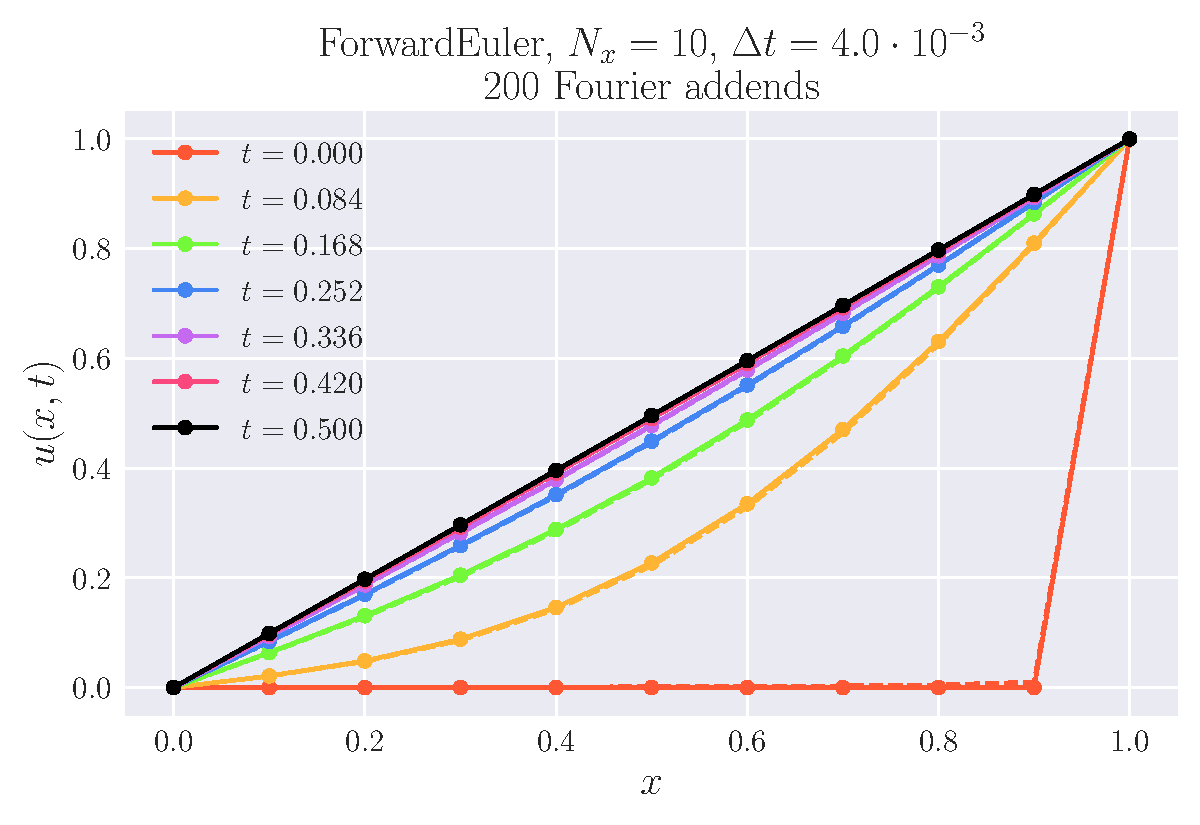
\includegraphics[width=\linewidth]{ForwardEuler-Nt125-dt4_0e-03-Nx10.pdf}
  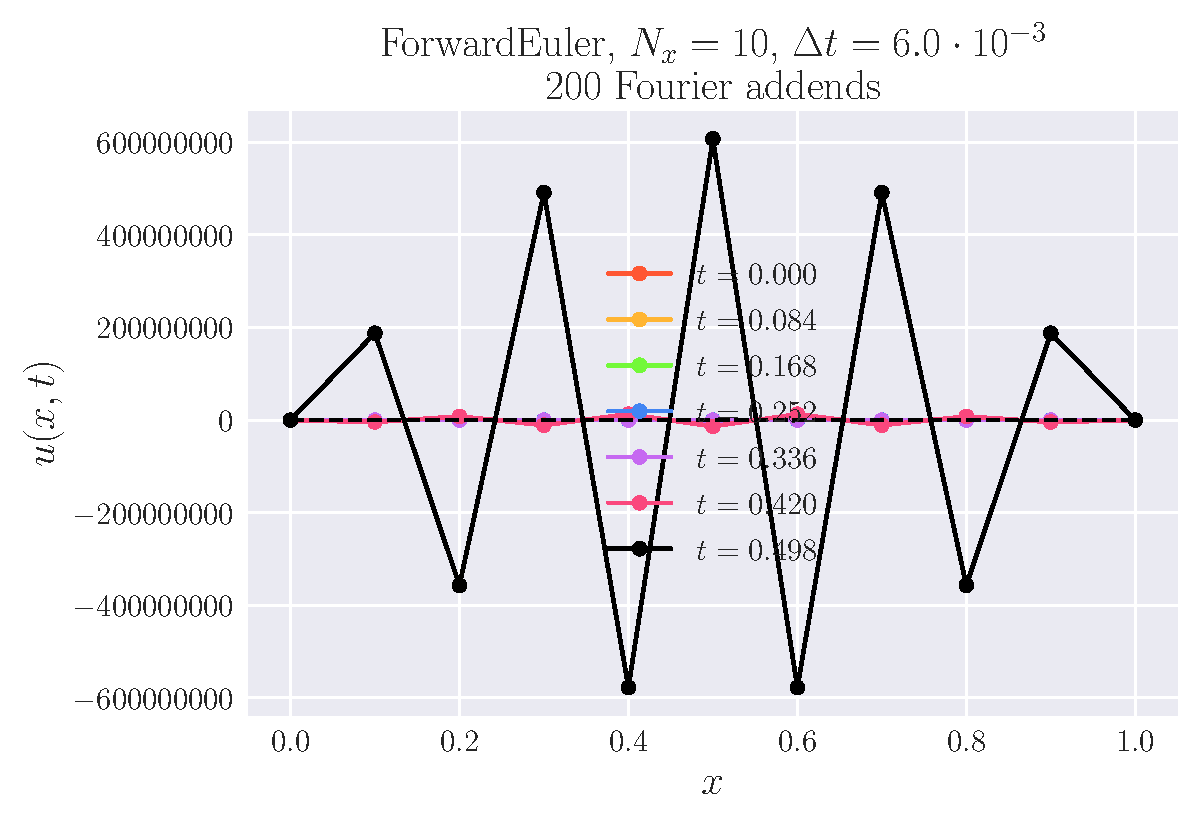
\includegraphics[width=\linewidth]{ForwardEuler-Nt83-dt6_0e-03-Nx10.pdf}
  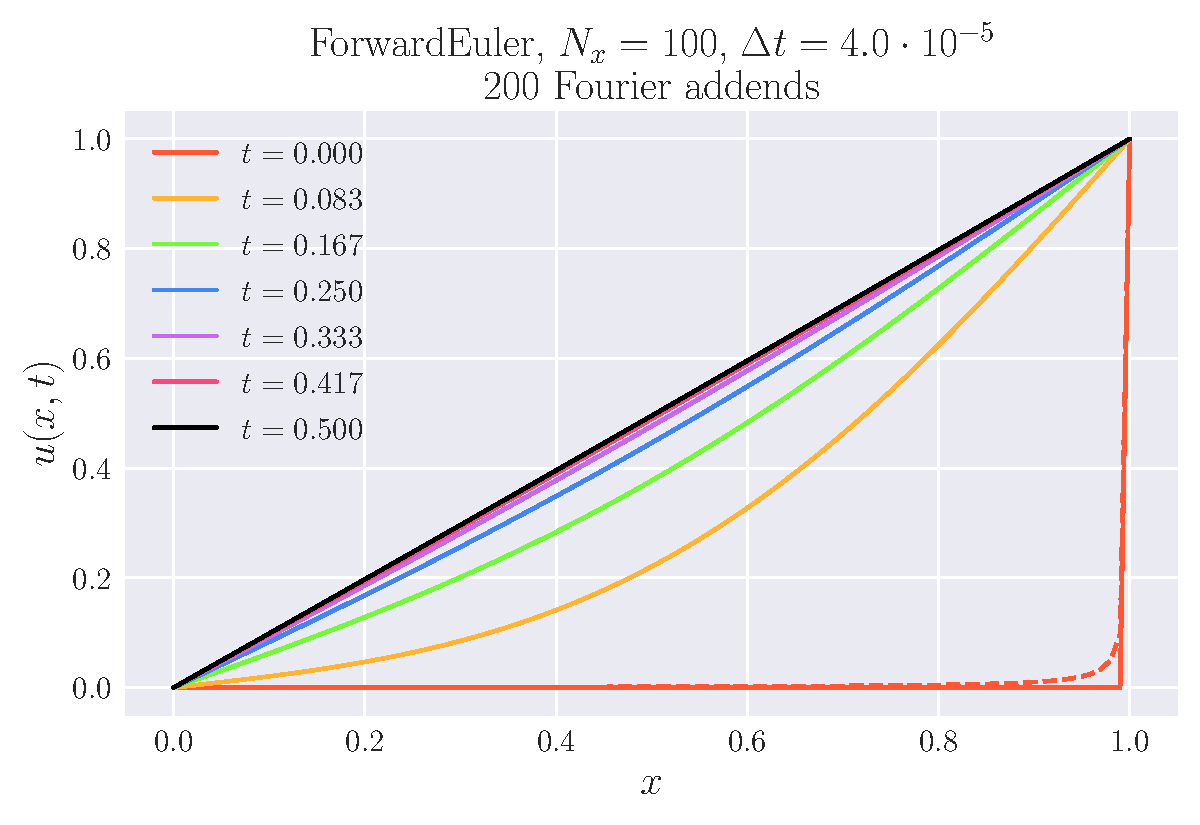
\includegraphics[width=\linewidth]{ForwardEuler-Nt12499-dt4_0e-05-Nx100.pdf}
  \caption{\(u(x, t)\) as a function of \(x\) calculated using the Forward Euler algorithm. The dashed lines show the analytical results, calculated with 200 addends in the Fourier sum in equation \eqref{eq:exact_solution_1D}. The different colors denote the solution at different times. The top two figures show the solution with $N_x = 10$, that is, eleven grid points with a distance \(\Delta x = 1/10\) between. The bottom figure shows \(N_x = 100\), giving \(\Delta x = 1/100\). The first and third figure are produced with the stability condition satisfied (\(\Delta t / \Delta x^2 = 0.4\)), whereas the second has \(\Delta t / \Delta x^2 = 0.6\).}
  \label{fig:ForwardEuler}
\end{figure}

Figure \ref{fig:ForwardEuler_error} shows the error for different number of integration points and values of \(\Delta t\). Since the error for \(\Delta x = 1/10\) and \(\Delta t / \Delta x^2 = 0.6\) is obviously very large (see the second plot in figure \ref{fig:ForwardEuler}), we have chosen to include here the errors for \(\Delta t / \Delta x^2 = 0.4\) (the first and third plot) and \(\Delta t / \Delta x^2 = 0.5\) (the second plot). The first two plots have \(N_x = 10\), i.e. eleven integration points, and the third plot has \(N_x = 100\). Different colors correspond to different times. The mean absolute percentage error (MAPE) can be read from the title for the different times.
\begin{figure}
  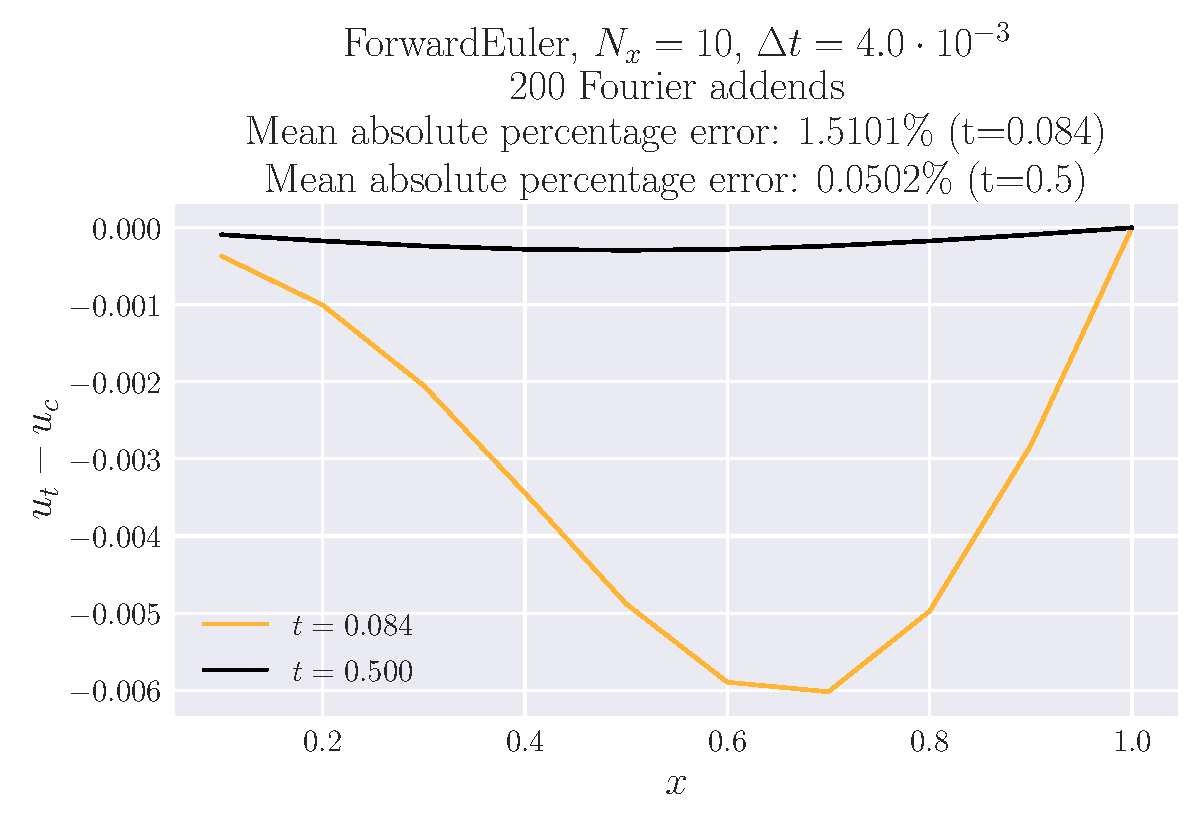
\includegraphics[width=\linewidth]{ForwardEuler-Nt125-dt4_0e-03-Nx10-Error.pdf}
  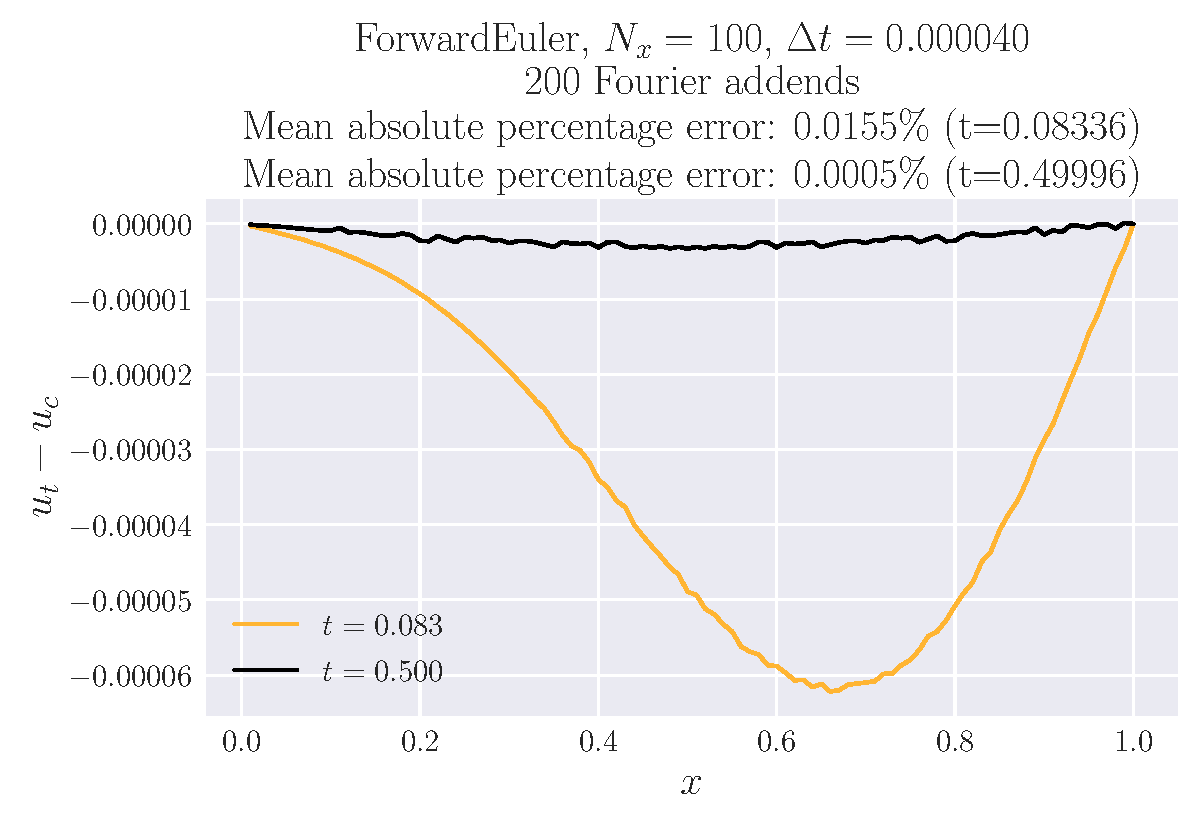
\includegraphics[width=\linewidth]{ForwardEuler-Nt12499-dt4_0e-05-Nx100-Error.pdf}
  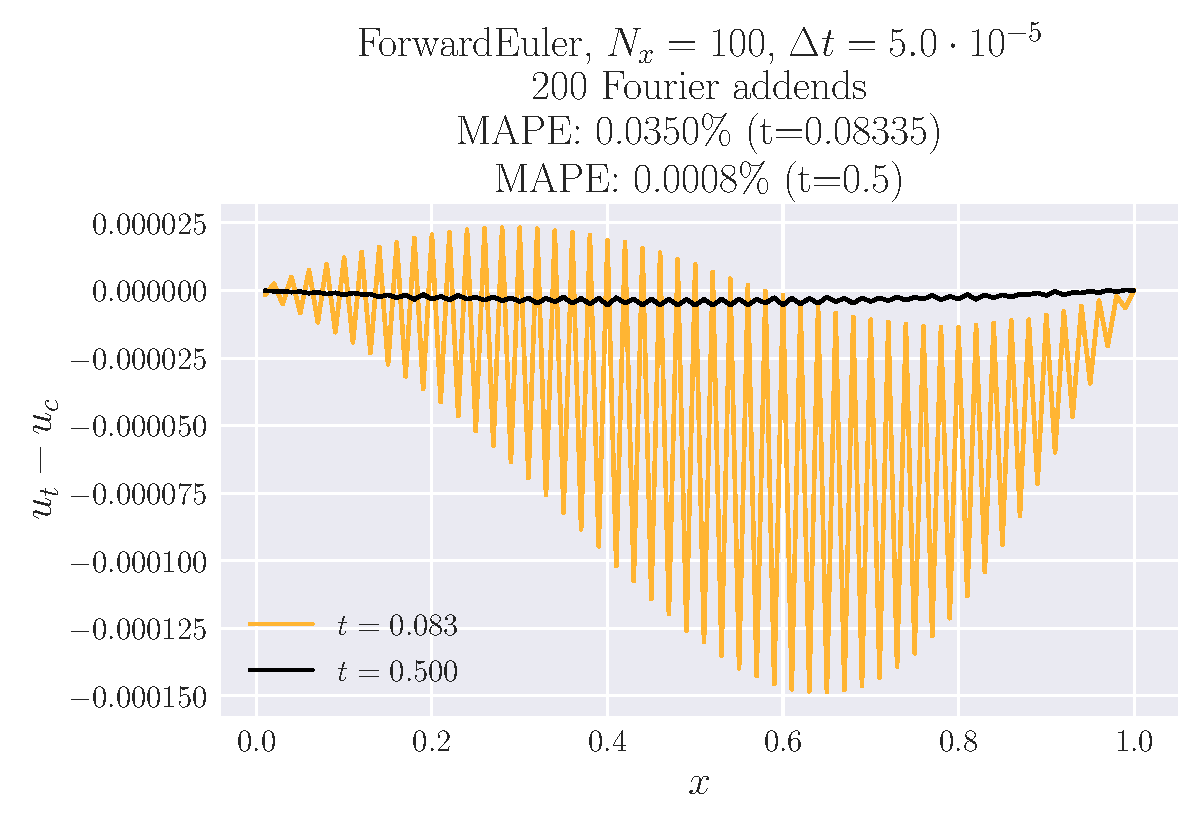
\includegraphics[width=\linewidth]{ForwardEuler-Nt10000-dt5_0e-05-Nx100-Error.pdf}
  \caption{The error for different number of integration points and values of \(\Delta t\) for the Forward Euler algorithm. Different colors correspond to different times. The mean absolute percentage error (MAPE) can be read from the title for the different times. The first and third plot have \(\Delta t / \Delta x^2 = 0.4\) and the second has \(\Delta t / \Delta x^2 = 0.5\). The first two plots have \(N_x = 10\), i.e. eleven integration points, and the third plot has \(N_x = 100\).}
  \label{fig:ForwardEuler_error}
\end{figure}

Figure \ref{fig:BackwardEuler_error} shows the difference between the computed values \(u_c(x, t)\) and the theoretical values \(u_t(x, t)\) as a function of \(x\) calculated using the Backward Euler algorithm. The first plot is made with \(N_x = 10\) and thus \(\Delta x = 1/10\). For the second and third plot, we have \(N_x = 100\) and \(\Delta x = 1/100\). For the first two plots we have used a value of \(\Delta t\) such that \(\Delta t / \Delta x^2 = 0.4\), i.e. the stability conditions for the explicit scheme were satisfied. In the third plot, we used a value of \(\Delta t\) such that \(\Delta t / \Delta x^2 = 0.6\) and the stability condition was not satisfied. Different colors correspond to different times. The mean absolute percentage error (MAPE) can be read from the title for the different times.
Figure \ref{fig:CrankNicolson_error} shows the same for the Crank-Nicolson scheme.

\begin{figure}
  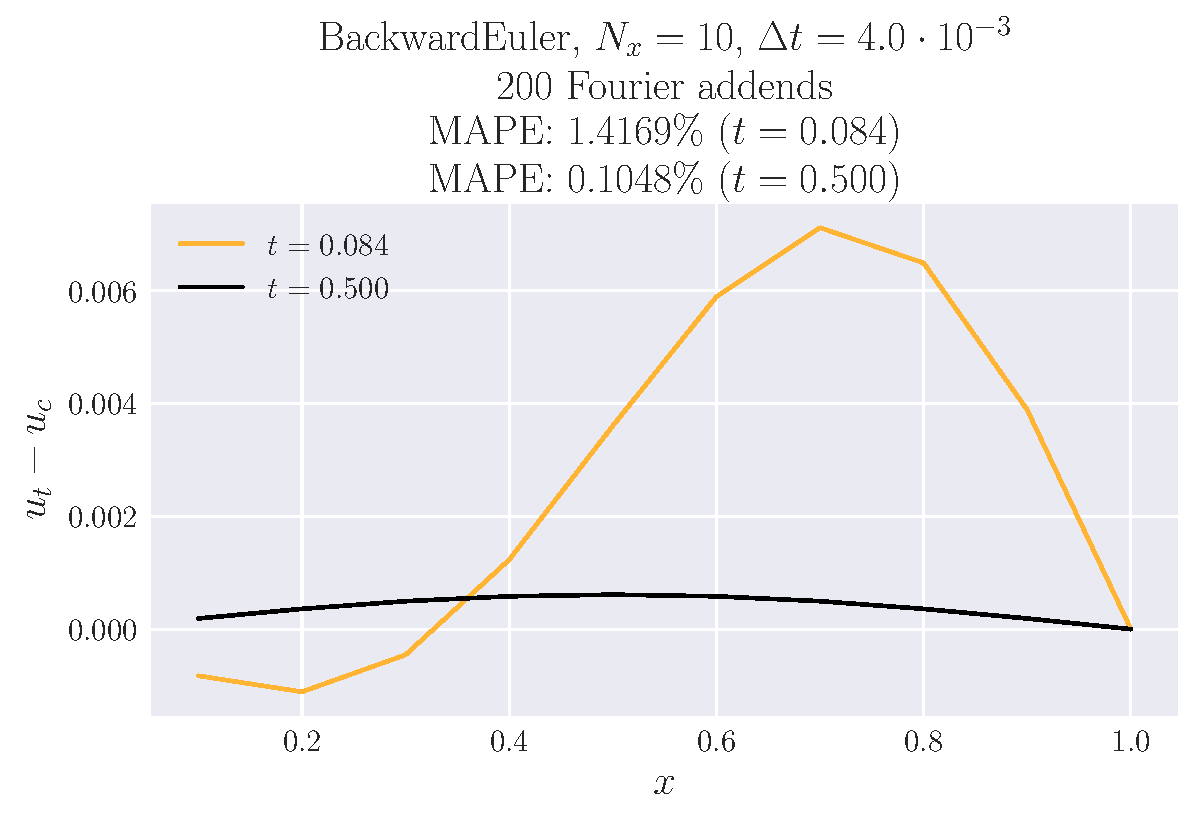
\includegraphics[width=\linewidth]{BackwardEuler-Nt125-dt4_0e-03-Nx10-Error.pdf}
  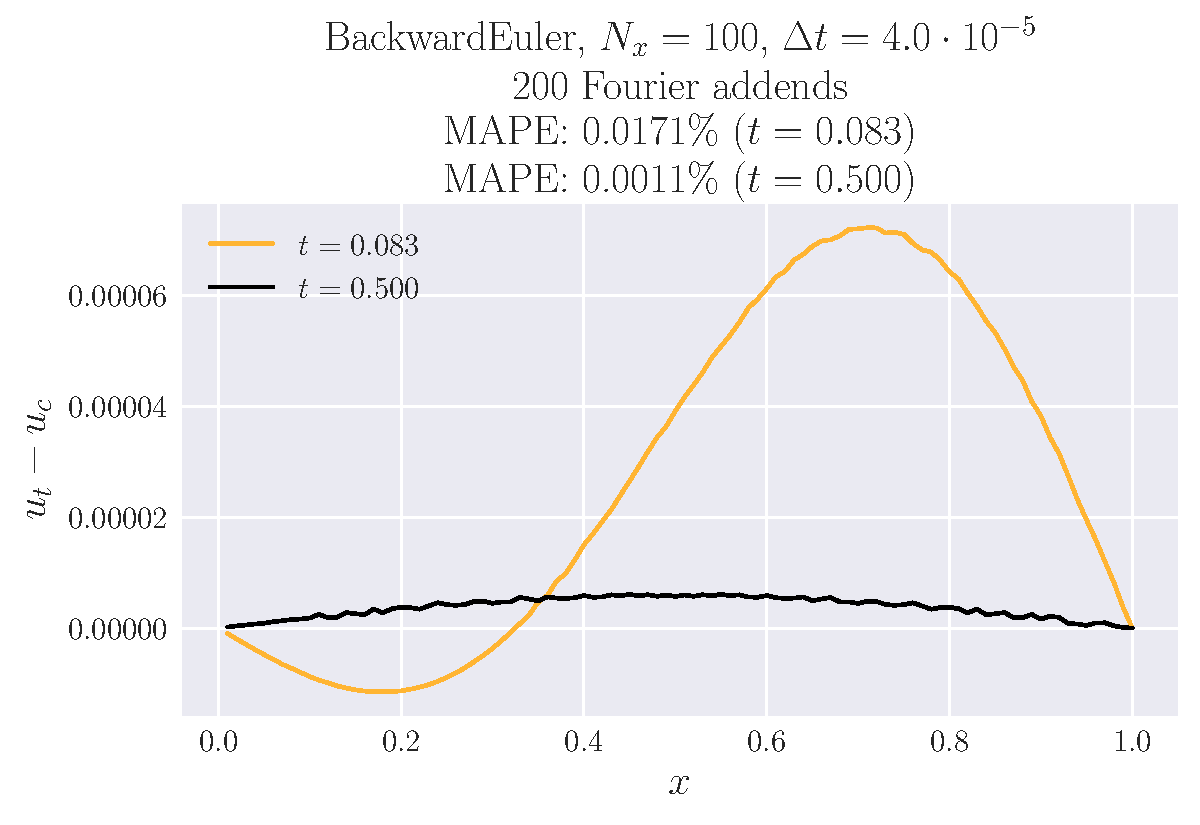
\includegraphics[width=\linewidth]{BackwardEuler-Nt12499-dt4_0e-05-Nx100-Error.pdf}
  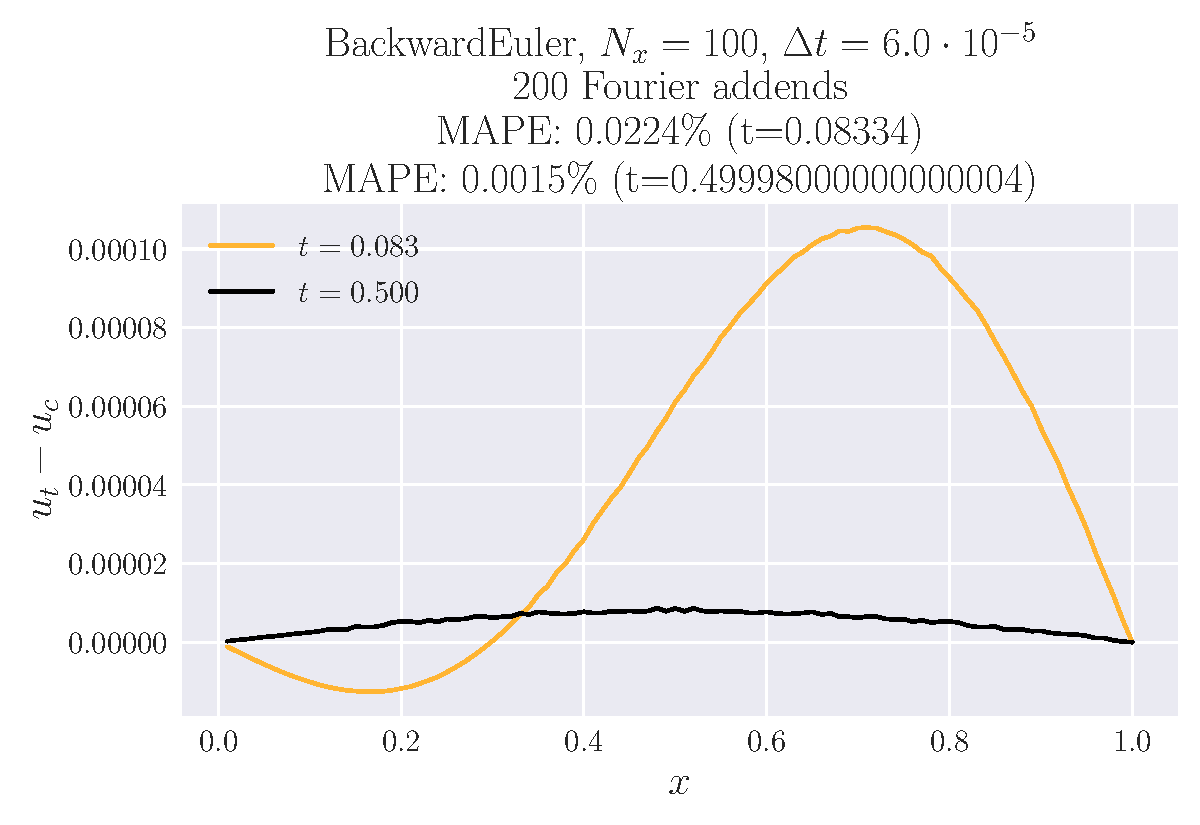
\includegraphics[width=\linewidth]{BackwardEuler-Nt8333-dt6_0e-05-Nx100-Error.pdf}
  \caption{The difference between the computed values \(u_c(x, t)\) and the theoretical values \(u_t(x, t)\) as a function of \(x\) calculated using the Backward Euler algorithm. The first plot is made with \(N_x = 10\) and thus \(\Delta x = 1/10\). For the second and third plot, we have \(N_x = 100\) and \(\Delta x = 1/100\). For the first two plots we have used a value of \(\Delta t\) such that \(\Delta t / \Delta x^2 = 0.4\). In the third plot, we used a value of \(\Delta t\) such that \(\Delta t / \Delta x^2 = 0.6\). Different colors correspond to different times. The mean absolute percentage error (MAPE) can be read from the title for the different times.}
  \label{fig:BackwardEuler_error}
\end{figure}
\begin{figure}
  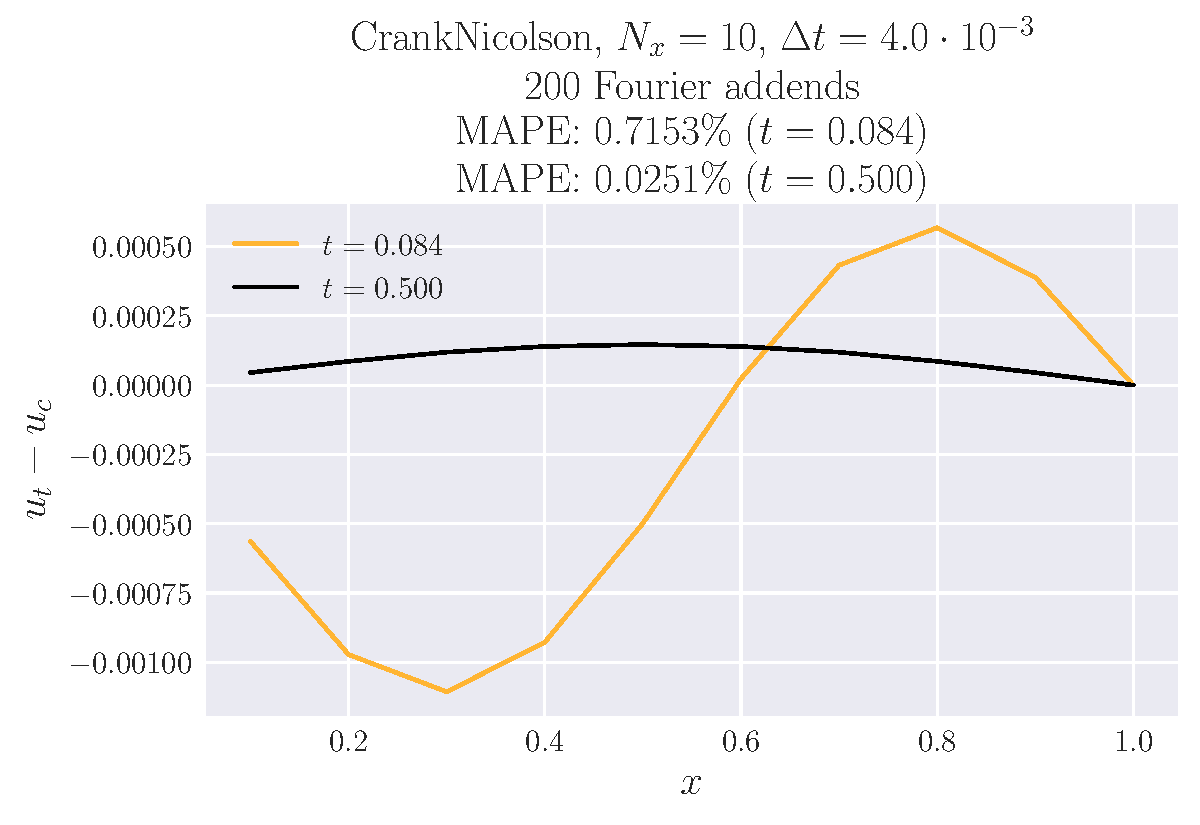
\includegraphics[width=\linewidth]{CrankNicolson-Nt125-dt4_0e-03-Nx10-Error.pdf}
  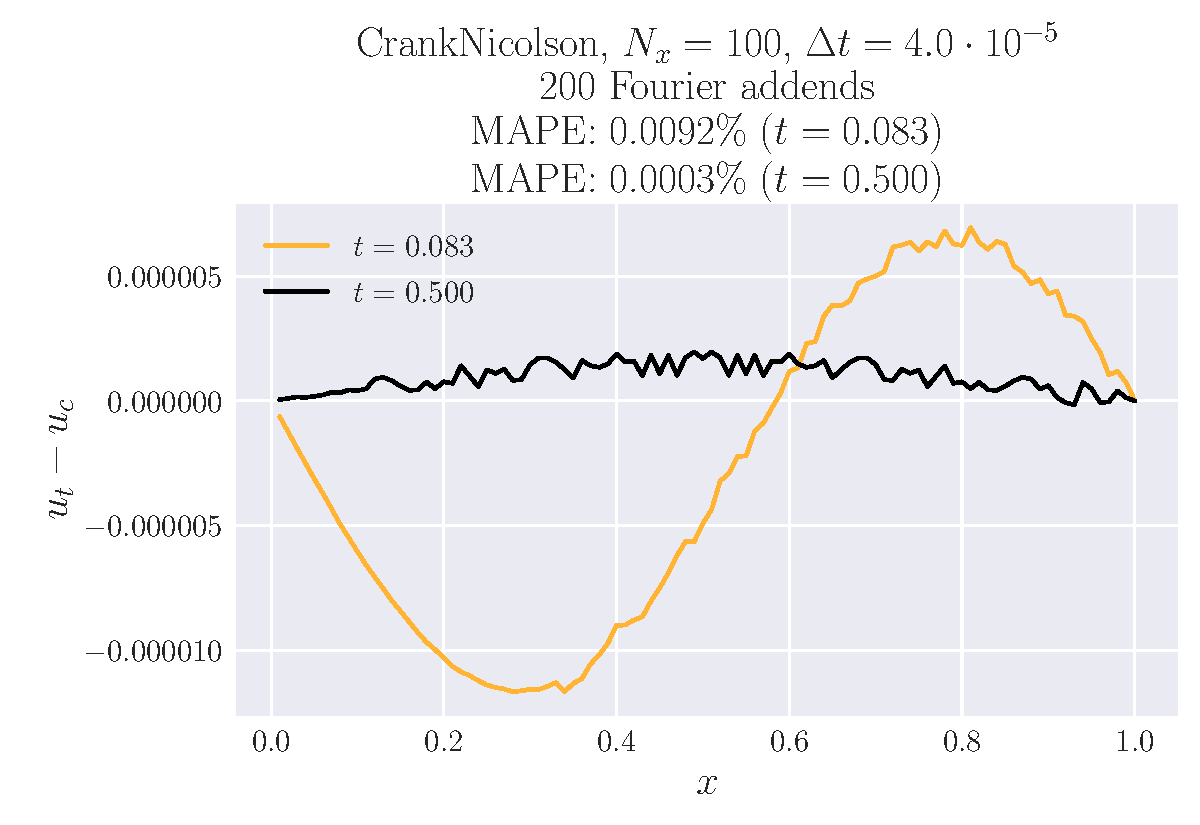
\includegraphics[width=\linewidth]{CrankNicolson-Nt12499-dt4_0e-05-Nx100-Error.pdf}
  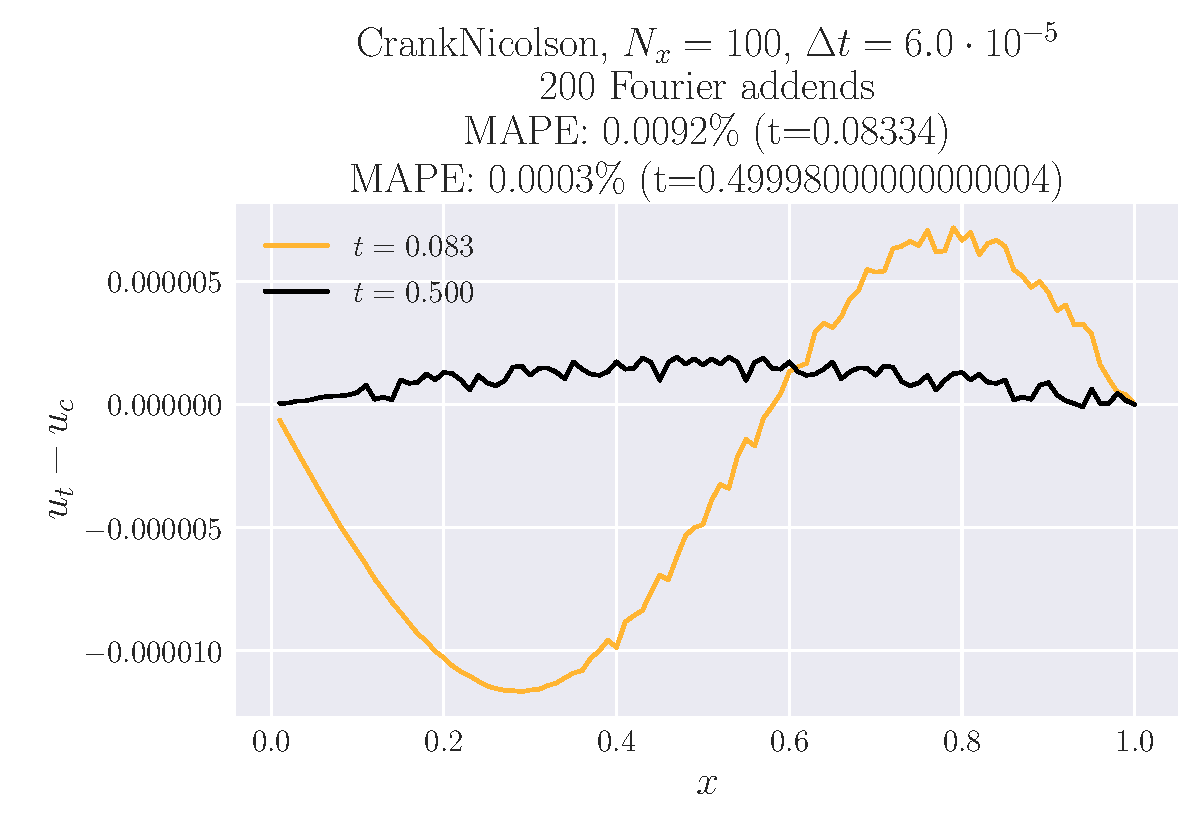
\includegraphics[width=\linewidth]{CrankNicolson-Nt8333-dt6_0e-05-Nx100-Error.pdf}
  \caption{The difference between the computed values \(u_c(x, t)\) and the theoretical values \(u_t(x, t)\) as a function of \(x\) calculated using the Crank-Nicolson algorithm. The first plot is made with \(N_x = 10\) and thus \(\Delta x = 1/10\). For the second and third plot, we have \(N_x = 100\) and \(\Delta x = 1/100\). For the first two plots we have used a value of \(\Delta t\) such that \(\Delta t / \Delta x^2 = 0.4\). In the third plot, we used a value of \(\Delta t\) such that \(\Delta t / \Delta x^2 = 0.6\). Different colors correspond to different times. The mean absolute percentage error (MAPE) can be read from the title for the different times.}
  \label{fig:CrankNicolson_error}
\end{figure}

Plots showing the actual values of \(u(x, t)\) as a function of \(x\) are not included in the report as they are visually indistinguishable from the last plot in figure \ref{fig:ForwardEuler}. The can be viewed in our GitHub repository previously linked to, and will be automatically produced by the code.

In figure \ref{fig:3D} we have plotted the analytical and computed results for stable and unstable conditions (equation \eqref{eq:2D_von_neumann_stability} satisfied and not). The top four plots are the stable solutions, at four different times. The bottom four are the unstable results at the same times. Above all of them we have plotted the analytical solution with a black mesh plot. To produce the analytical results we have used equation \eqref{eq:2D_closed_sol} with $n = m = 50$ (larger values did not yield better results). Note that the unstable result has very large oscillations.

Figure \ref{fig:3D_error} shows the difference between the analytical and stable computed result. We also made a table \ref{tab:error_2D} that shows MAPE (calculated using equation \eqref{eq:MAPE}) for the stable and unstable solution, at the different time steps displayed in figure \ref{fig:3D}. There was no point plotting the difference between unstable and theoretical solution, because it look identical to the unstable results in figure \ref{fig:3D}.
\begin{figure*}[!htb]
	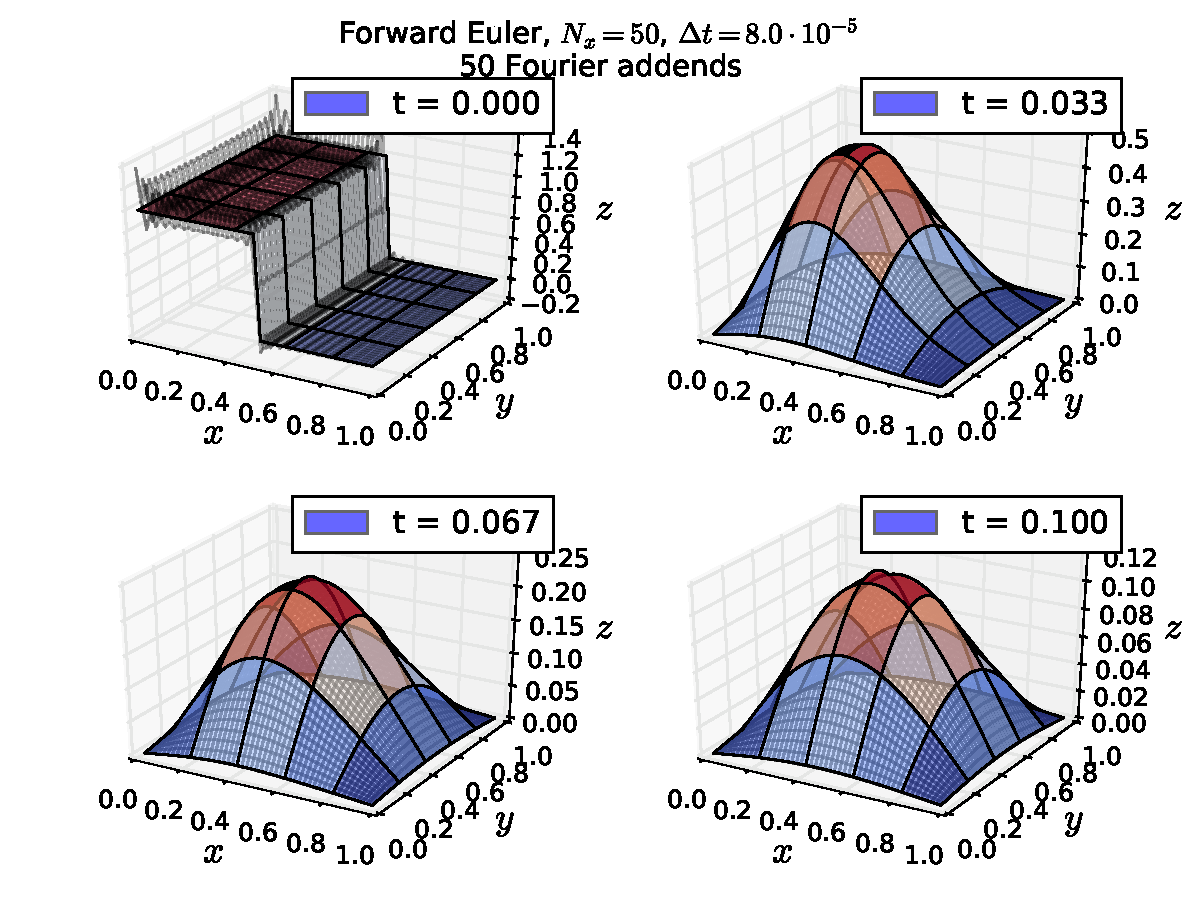
\includegraphics[width=16cm]{TwoDimensions-Nt1250-dt8_0e-05-Nx50.pdf}
	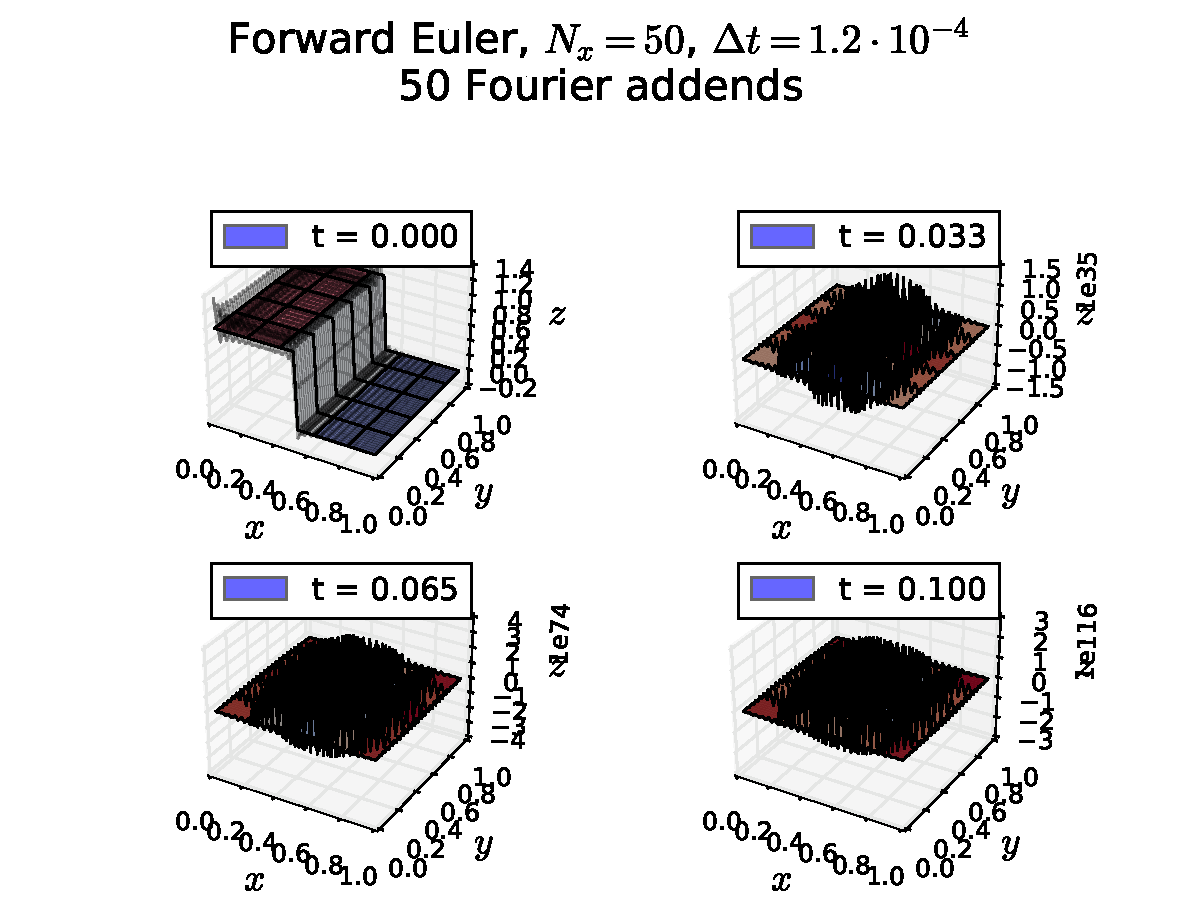
\includegraphics[width=16cm]{TwoDimensions-Nt833-dt1_2e-04-Nx50.pdf}
	\caption{In this figure you see the analytical and computed result for the two dimensional problem. The colored plot is the computed, and the black mesh plot is the analytical plot. The top four plots are the stable solutions, and the bottom four are the unstable ones. They are all plotted at the same time steps, $n=m50$ Fourier addends and number of integration points in $x-$ and $y-$direction.
	\label{fig:3D}}
\end{figure*}

\begin{figure*}[!htb]
	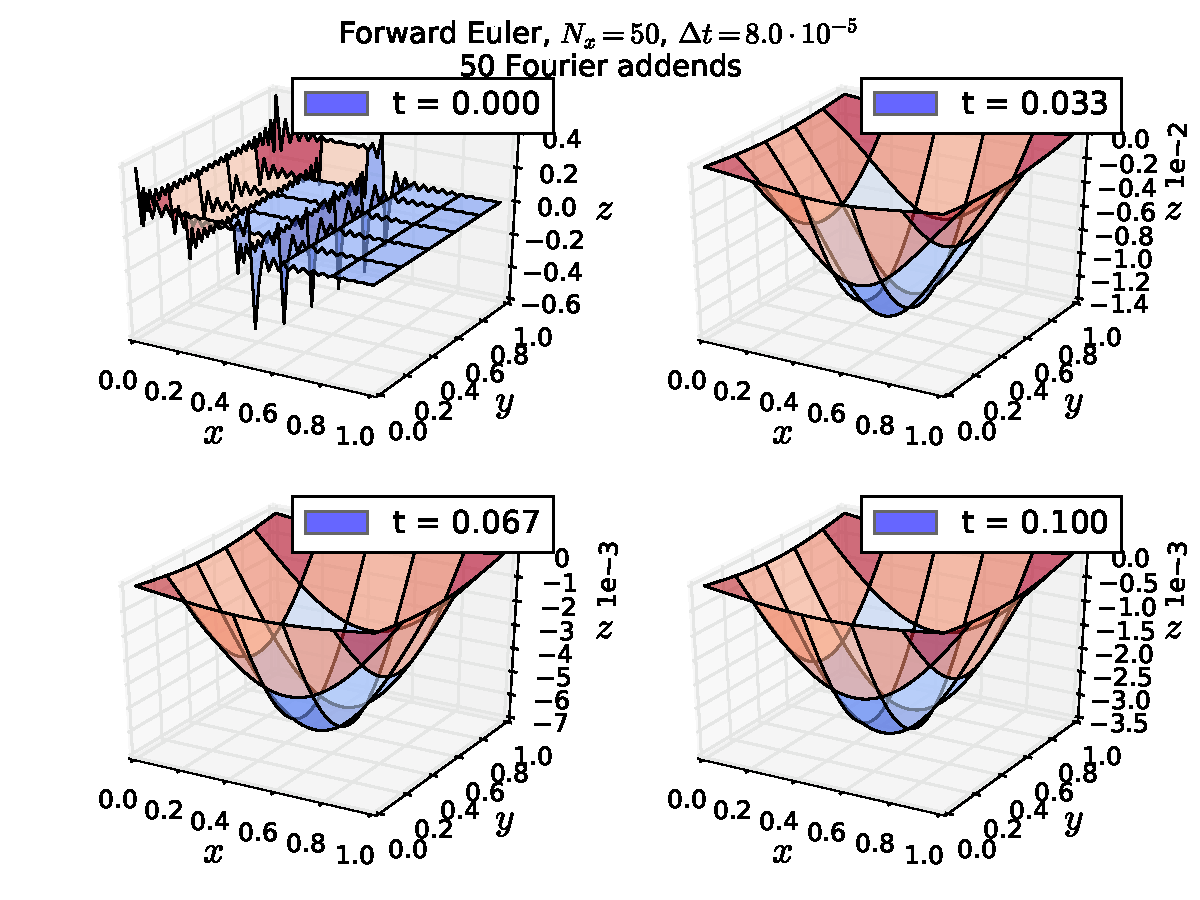
\includegraphics[width=16cm]{TwoDimensions-Nt1250-dt8_0e-05-Nx50-Error.pdf}
	\caption{In this figure we have plotted the difference between the theoretical and stable computed values. We used $n=m=50$ Fourier addends, and plotted the difference for three different time steps, the same as in figure \ref{fig:3D}.
	\label{fig:3D_error}}
\end{figure*}


\begin{table}[!htb] %\cellcolor{grey!20}
	\begin{tabular}{|l|l|l|l|} \hline
		Unstable&& Stable &\\ \hline
		MAPE [\%]   & Time  & MAPE [\%]  & Time  \\ \hline
		0.039               & 0.000 & 0.039 & 0.000 \\ \hline
		3.95e+34               & 0.033 & 0.0049 & 0.033 \\ \hline
		1.27e+74               & 0.067 & 0.0026 & 0.067 \\ \hline
		9.38e+115              & 0.100 & 0.0013 & 0.100 \\ \hline
	\end{tabular}
	\caption{In this table we have calculated the MAPE (in percent) for the stable and unstable computed values, and for different time steps. The first two columns are the stable values, and the second two unstable ones.
	\label{tab:error_2D}}
\end{table}

\section{Discussion}

From figure \ref{fig:ForwardEuler} we see very clearly the importance of satisfying the stability condition for the explicit Forward Euler scheme. The first and third plots show the function changing rapidly in the initial stage and then converging more and more slowly to a stationary state (which is a linear function of \(x\)), exactly as we expected. The second plot shows disastrous oscillations that leave the computed solution entirely useless. The function values oscillate between \(\pm 6 \cdot 10^8\), when we know for certain that the correct solution should always be in the range [0, 1]. This was caused by simply increasing the value of \(\Delta t\) by 50\% such that \(\Delta t / \Delta x^2\) changes from 0.4 to 0.6. It is therefore very important to be aware of and consider the stability condition when using the Forward Euler algorithm.

We see from figure \ref{fig:ForwardEuler_error} that the error is reduced by approximately a factor of 100 when increasing the number of integration steps from 10 to 100, while also adjusting \(\Delta t\) such that \(\Delta t / \Delta x^2 = 0.4\) in both cases. This also seems to hold true for the mean absolute percentage error. The bottom plot, where \(\Delta t / \Delta x^2 = 0.5\) just satisfies the stability condition, we already see the start of the oscillations so clearly visible in figure \ref{fig:ForwardEuler}. The oscillations cause mean absolute percentage error to be over twice as large for \(t = 0.083\) (0.0350\% vs. 0.0155\%). We have verified that the error is not caused by too few addends in the Fourier sum by increasing the number from 200 to 400. To the degree of precision with which we have presented our results, the values for the errors were identical.
From the stability condition, one might presume that \(\Delta t / \Delta x^2 = 0.5\) would be a safe choice. Indeed, the results are nowhere near as bad as with \(\Delta t / \Delta x^2 = 0.6\), but we do see the a tendency of the same problem with oscillations. It seems therefore that the wise approach is to make sure that you strictly satisfy the stability condition (\(\Delta t / \Delta x^2 < 0.5\)) in order to be confident in your results.

The results produced by the Backward Euler and Crank-Nicolson schemes were not affected by the value of \(\Delta t / \Delta x^2\) in the same way as the Forward Euler algorithm. From figures \ref{fig:BackwardEuler_error} and \ref{fig:CrankNicolson_error} we see that all the values for the error is decreased by a factor of approximately 80-100 when increasing the number of integration points from 10 to 100 while keeping the value \(\Delta t / \Delta x^2 = 0.4\) constant.

Like we observed in the two-dimensional case, satisfying the stability condition is paramount to having good results. Looking at table \ref{tab:error_2D} we see that the MAPE is around $10^{34-115}$\%, which means we are far away from the actual solution. When satisfying the condition however, we notice (also from table \ref{tab:error_2D}) good correlation between the actual values (MAPE of around $10^{-3}$\%). We tried to increase the number of Fourier addends, however saw no change in error, meaning the actual solution should be accurate. Another thing which we observed in the one dimensional problem was oscillations in the computed values. It seems to be a product of not satisfying the stability conditions. If you don't know the stability conditions, this could be something to be vary of.

Each algorithm have their strength. Backward Euler and Crank-Nicolson are both unconditionally stable, giving it a clear edge over forward Euler. If stability conditions are not satisfied, the unconditionally algorithms still gave decent results, forward Euler however gave results with no resemblance of the actual result. On the other hand, when stability conditions were satisfied, forward performed similar to backward Euler in our tests. For $N_x = 10$, $N_x =100$ and $\Delta t = 4\cdot 10^{-3}$ forward Euler had around the same values of MAPE as backward. When $N_x = 10$ forward had MAPE$=0.0155\%$ ($t = 0.83$) and MAPE=$0.0005\%$ ($t=0.50$), backward had MAPE$=1.4169\%$ ($t = 0.83$) and MAPE=$0.1048\%$ ($t=0.50$). Looking at the plots \ref{fig:ForwardEuler_error} and \ref{fig:BackwardEuler_error}, they also seem similar. They both stray away from zero equally far (around $6\cdot10^{-3}$). We notice the same trend for $N_x = 100$, implying that forward is equal to backward Euler when stability conditions are satisfied. Crank-Nicolson outperformed forward and backward in all cases. The MAPE-percentages were lower for all cases, also looking at the error-plots, they do not stray as far away from zero as forward and backward. This is expected, as we mentioned in the theory section backward and forward has errors $O(\Delta t)$ and $O(\Delta x^2)$ and Crank-Nicolson errors $O(\Delta t^2)$ and $O(\Delta x^2)$. When considering ease of implementation, forward and backwards Euler comes on top. Forward Euler is notoriously easy to implement, and as we have seen in this report, it gives good solutions when stability conditions are satisfied.

\subsection*{Code optimization}

We did see a significant speed-up from the parallelization, the code was approximately twice as fast with eight cores as with one core. Given more time, there are several avenues we could have explored to improve on our solution, both to reduce memory consumption and computing time.

One possibility is to use only one-dimensional arrays for storing our results. We have done this to some extent in our code by representing the three-dimensional array of results (\(\text{timesteps} \times x \times y\)) as a two-dimensional array. Here, one one-dimensional sub-array represents the matrix in the \(x, y\)-plane at one time step. We could have gone further and represented the entire result array with a one-dimensional array, which is generally thought to reduce computing times. We have made a working attempt at this, which can be viewed on a developmental branch in our GitHub repository\footnote{https://github.com/sigurdru/FYS3150/tree/vegard\_test/Project5/code}. We were surprised to find that this code was actually slower than our first implementation. Simple timing indicated that the computing time was around 50\% greater. It is possible that our way of indexing this one-dimensional array was sub-optimal and it is definitely something that would be interesting to investigate further.

A possible improvement, mainly with regard to memory usage, is the way we keep track of which diagonals have been calculated by the different cores. This is now implemented as a boolean array with one value for each diagonal of each time step that is simultaneously being calculated. This is possibly ineff SKAL DETTE MED?

Another alteration, which most certainly would increase the efficiency of our program, is to allow each core to calculate values for more than one time step between each time the threads are gathered and the result matrix reset. In our implementation, we let every core calculate the values for the entire grid in one time step each. After all the cores have completed this task, the threads are gathered, the result array is reset and the process is repeated. To split and gather the threads introduces overhead and takes time. By allowing each core to calculate more than one time step each before the reset, we could easily reduce this overhead cost manyfold over the course of the total calculation. If we for instance use two cores for calculation, then allowing the first core to calculate the first and third next time steps, and the second core to calculate the second and fourth next time steps before the reset would half the number of times the threads are split and gathered. This would require more memory as the result array would have to be larger. Representing the results for all time steps in one large array, while probably the fastest approach, would in most cases require more memory than is available. Our solution would have to land somewhere in-between, using enough memory to allow each core to calculate several time steps each, but not exhaust the memory resources of the computer. This tradeoff between memory consumption and computational efficiency is a recurring theme in computer science.

There are also possible improvements to be made with the way we reset the values in the result matrix. We store the results in a matrix where each row corresponds to a specific time step. During reset, the values of the first row are updated to the values of the last row. The values of the other rows are set to zero. Firstly, while setting to zero the values that should later be updated is practical for troubleshooting, it is highly unnecessary and inefficient during larger calculations. The values will later be updated and setting them all to zero is simply a costly operation that in the end serves no purpose. Secondly, we probably do not need to move the elements from the first row to the last row one by one. We could change the pointer to the first row to instead point to the last row and vice versa. This would save a lot of indexing and memory handling during the reset, and could potentially reduce the computing time by a considerable amount.



\section{Conclusion}

Conclusion



\onecolumngrid
\vspace{1cm} % some extra space

\begin{thebibliography}{}
\bibitem[]{lectures2015} Morten Hjorth-Jensen, Computational Physics, Lecture Notes Fall 2015, August 2015, https://github.com/CompPhysics/ComputationalPhysics/blob/master/doc/Lectures/lectures2015.pdf.
\bibitem[]{2D_diffusion} Ryan C. Daileda, Trinity University, Partial Differential Equations, March 6, 2012, http://ramanujan.math.trinity.edu/rdaileda/teach/s12/m3357/lectures/lecture\_3\_6\_short.pdf.
\bibitem[]{MiT} massachusetts institute of technology, Numerical Methods for Partial Differential Equations, March 31. 2009, https://ocw.mit.edu/courses/mathematics/18-336-numerical-methods-for-partial-differential-equations-spring-2009/lecture-notes/MIT18\_336S09\_lec14.pdf.
\bibitem{PDE_book} Tveito, Aslak and Winther, Ragnar, Introduction to Partial Differential Equations A Computational Approach, 2005.

\end{thebibliography}


\section{Appendix}

\subsection{Derivation of equation for the Crank-Nicolson scheme} \label{sect:Crank-Nicolson_derivation}

Again we define
\begin{equation*}
  \alpha = \frac{\Delta t}{(\Delta x)^2}
\end{equation*}
Inserting the approximations of $u_t$ and $u_{xx}$ stated in the Theory section into our differential equation, we get
\begin{align*}
  u_t &= u_{xx} \\
  \frac{u_{i, j+1} - u_{i, j}}{\Delta t}
    &= \frac{1}{2 \Delta x^2} \bigg(u_{i+1, j} - 2u_{i,j} + u_{i-1, j}
      + u_{i+1, j + 1} - 2u_{i, j + 1} + u_{i - 1, j + 1} \bigg) \\
  u_{i, j+1} - u_{i, j} &= \frac{\alpha}{2} \bigg(u_{i+1, j} - 2u_{i,j} + u_{i-1, j}
      + u_{i+1, j+1} - 2u_{i, j+1} + u_{i-1, j+1} \bigg) \\
  u_{i, j+1} - \frac{\alpha}{2} \bigg( u_{i+1, j+1} - 2u_{i, j+1} + u_{i-1, j+1} \bigg)
    &= u_{i, j} + \frac{\alpha}{2} \bigg(u_{i+1, j}  - 2u_{i,j} + u_{i-1, j} \bigg) \\
  2 u_{i, j+1} - \alpha u_{i+1, j+1} + 2 \alpha u_{i, j+1} - \alpha u_{i-1, j+1}
    &= 2 u_{i, j} + \alpha u_{i+1, j}  - 2 \alpha u_{i,j} + \alpha u_{i-1, j} \\
  - \alpha u_{i-1, j+1} + 2 (1 + \alpha) u_{i, j+1} - \alpha u_{i+1, j+1}
    &= \alpha u_{i-1, j}  + 2 (1 - \alpha) u_{i,j} + \alpha u_{i+1, j} \numberthis \label{eq:CrankNicolson}
\end{align*}
Written out explicitly for all $i$, the equation reads
\begin{align*}
  - \alpha u_{0, j+1} + 2 (1 + \alpha) u_{1, j+1} - \alpha u_{2, j+1}
    &= \alpha u_{0, j}  + 2 (1 - \alpha) u_{1,j} + \alpha u_{2, j} \\
  - \alpha u_{1, j+1} + 2 (1 + \alpha) u_{2, j+1} - \alpha u_{3, j+1}
    &= \alpha u_{1, j}  + 2 (1 - \alpha) u_{2,j} + \alpha u_{3, j} \\
    \vdots \\
  - \alpha u_{n-3, j+1} + 2 (1 + \alpha) u_{n-2, j+1} - \alpha u_{n-1, j+1}
    &= \alpha u_{n-3, j}  + 2 (1 - \alpha) u_{n-2,j} + \alpha u_{n-1, j} \\
  - \alpha u_{n-2, j+1} + 2 (1 + \alpha) u_{n-1, j+1} - \alpha u_{n, j+1}
    &= \alpha u_{n-2, j}  + 2 (1 - \alpha) u_{n-1,j} + \alpha u_{n, j}
\end{align*}

Similar to the case of Backward Euler, this set of equations can be rearranged as follows
\begin{align*}
  2 (1 + \alpha) u_{1, j+1} - \alpha u_{2, j+1}
    &= \alpha u_{0, j}  + 2 (1 - \alpha) u_{1,j} + \alpha u_{2, j} + \alpha u_{0, j+1} \\
  - \alpha u_{1, j+1} + 2 (1 + \alpha) u_{2, j+1} - \alpha u_{3, j+1}
    &= \alpha u_{1, j}  + 2 (1 - \alpha) u_{2,j} + \alpha u_{3, j} \\
    \vdots \\
  - \alpha u_{n-3, j+1} + 2 (1 + \alpha) u_{n-2, j+1} - \alpha u_{n-1, j+1}
    &= \alpha u_{n-3, j}  + 2 (1 - \alpha) u_{n-2,j} + \alpha u_{n-1, j} \\
  - \alpha u_{n-2, j+1} + 2 (1 + \alpha) u_{n-1, j+1}
    &= \alpha u_{n-2, j}  + 2 (1 - \alpha) u_{n-1,j} + \alpha u_{n, j} + \alpha u_{n, j+1}
\end{align*}
We can define the vector $\vc b_j$ to hold the values on the right side of each of these equations:
\begin{equation}
  \label{def:vector_b_CrankNicolson_appendix}
  \vc b_j =
  \begin{bmatrix}
    \alpha u_{0, j}  + 2 (1 - \alpha) u_{1,j} + \alpha u_{2, j} + \alpha u_{0, j+1} \\
    \alpha u_{1, j}  + 2 (1 - \alpha) u_{2,j} + \alpha u_{3, j} \\
      \vdots \\
    \alpha u_{n-3, j}  + 2 (1 - \alpha) u_{n-2,j} + \alpha u_{n-1, j} \\
    \alpha u_{n-2, j}  + 2 (1 - \alpha) u_{n-1,j} + \alpha u_{n, j} + \alpha u_{n, j+1}
  \end{bmatrix}
\end{equation}
Using this and the definition of the vector $\vc v_j$ from \eqref{def:vector_v}, we can write the set of equations as
\begin{equation*}
  \vc A \vc v_j = \vc b_j
\end{equation*}
where the matrix $\vc A$ is a tridiagonal matrix with $2 (1 + \alpha)$ on the diagonal and $-\alpha$ directly above and below the diagonal.


\end{document}
